\documentclass{book}
\usepackage[utf8]{inputenc}
\usepackage{cmap}
\usepackage[T1]{fontenc}
\usepackage[italian]{babel}
\usepackage{graphicx}
\usepackage{placeins}
\usepackage{url}
\usepackage{tabularx}
\usepackage{ragged2e}
\newcolumntype{Y}{>{\RaggedRight\arraybackslash}X}
\newcolumntype{P}[1]{>{\RaggedRight\arraybackslash}p{#1}}
\usepackage{newunicodechar}
\usepackage{amsmath}
\usepackage{amssymb, amsfonts}
\newunicodechar{┌}{|}

\begin{document}

\chapter*{Introduzione}
\markboth{Introduzione}{Introduzione}

L'intelligenza artificiale trova spazio in attività quotidiane e professionali, offrendo strumenti con cui elaborare informazioni e affrontare compiti differenti. Tra questi, i modelli linguistici di grandi dimensioni, indicati con l'acronimo LLM (\textit{Large Language Models}), permettono di interagire attraverso il linguaggio naturale e possono affiancare l'utente nella scrittura, nella sintesi di testi e nell'organizzazione delle idee \cite{Korinek_2023}. Il loro interesse risiede anche nella possibilità di rendere accessibili queste funzioni mediante un'interazione diretta, nella quale una richiesta può essere precisata e sviluppata nel corso del dialogo.

Il valore di tali strumenti dipende dal modo in cui vengono utilizzati e dalla loro adeguatezza al compito. Le risposte devono essere esaminate alla luce delle informazioni disponibili e delle esigenze dell'attività svolta. L'impiego dell'intelligenza artificiale come supporto richiede quindi di comprenderne le capacità e i limiti, mantenendo un ruolo attivo nell'interpretazione dei risultati.

Le applicazioni dell'intelligenza artificiale comprendono anche l'analisi dei dati visivi. La visione artificiale sviluppa metodi per estrarre informazioni dalle immagini e riconoscere caratteristiche, oggetti o variazioni del loro aspetto. Nell'ambito industriale, queste capacità possono supportare il controllo di qualità attraverso l'identificazione di elementi che si discostano dalle caratteristiche attese di un prodotto \cite{Yang_et_al._2021,Cui_et_al._2023}.

La varietà dei materiali rende questo compito articolato. Una superficie può presentare una texture regolare oppure variazioni naturali di colore e tessitura; un oggetto può richiedere di considerare anche la forma e la disposizione delle sue parti. Le caratteristiche che definiscono la conformità dipendono pertanto dal materiale e dal prodotto osservato. Anche le anomalie assumono forme differenti: possono riguardare alterazioni cromatiche, tagli, pieghe, perforazioni o altri cambiamenti locali, con dimensioni e posizioni variabili. Distinguere un difetto da una variazione ammessa richiede una descrizione della normalità coerente con il contesto di osservazione \cite{Cui_et_al._2023}.

Un'ulteriore difficoltà riguarda la disponibilità di esempi. Quando le anomalie sono poco frequenti, raccogliere immagini che rappresentino tutte le possibili tipologie di difetto può risultare difficile. Inoltre, i campioni disponibili non esauriscono necessariamente le manifestazioni che potranno presentarsi in seguito. Questa condizione motiva l'interesse per metodi che apprendono le caratteristiche dei campioni normali e individuano, nelle nuove immagini, deviazioni rispetto alle regolarità apprese \cite{Pang_et_al._2021,Yang_et_al._2021}.

Da queste considerazioni nasce il presente project work, dedicato al rilevamento delle anomalie visive nell'ispezione industriale. Il lavoro confronta quattro modelli, CCW-SSIM, PaDiM, RD4AD e FastFlow, che adottano approcci differenti alla descrizione della normalità. La sperimentazione riguarda la categoria \texttt{leather} del dataset MVTec AD, scelta come caso di studio comune. La varietà dei materiali costituisce il contesto del problema; il confronto sperimentale si concentra invece su un unico materiale, per analizzare il comportamento delle pipeline nelle condizioni adottate.

La domanda che guida l'elaborato riguarda la capacità di questi approcci di riconoscere immagini difettose e di localizzare le regioni anomale. L'esame delle metriche è affiancato dalla lettura delle mappe prodotte, così da collegare i risultati numerici alle risposte osservabili nelle immagini. Il capitolo seguente introduce i concetti necessari a inquadrare il problema e i criteri con cui verrà valutato il confronto.

\chapter{Introduzione e definizione del problema}
\label{chap:introduzione}

L'\textbf{anomaly detection}, o rilevamento delle anomalie, consiste nell'identificare osservazioni che si discostano significativamente dal comportamento prevalente dei dati. Tali deviazioni possono suggerire la presenza di un meccanismo generativo differente e, nei contesti applicativi, segnalare eventi che richiedono un approfondimento \cite{Pang_et_al._2021}.

La difficoltà del problema dipende soprattutto da tre caratteristiche:
\begin{itemize}
    \item \textbf{scarsa conoscenza preliminare}: alcune tipologie di anomalia diventano note soltanto quando si manifestano;
    \item \textbf{eterogeneità}: anomalie diverse possono presentare caratteristiche visive o statistiche molto differenti;
    \item \textbf{rarità}: i campioni anomali sono spesso poco numerosi rispetto a quelli che descrivono il normale funzionamento.
\end{itemize}

Queste caratteristiche rendono difficile raccogliere esempi rappresentativi di tutti i difetti possibili. La ricerca sul rilevamento delle anomalie ha quindi sviluppato metodi capaci di apprendere la regolarità dei dati e di riconoscere deviazioni non necessariamente osservate durante l'addestramento. Tra le principali questioni aperte si distinguono \cite{Pang_et_al._2021}:
\begin{enumerate}
    \item \textbf{Sensibilità e falsi allarmi}. Un basso richiamo (\textit{recall}) indica che una parte delle anomalie non viene rilevata, producendo falsi negativi. Aumentare la sensibilità può però incrementare i falsi positivi, ossia i campioni normali segnalati come anomali. Il compromesso tra questi due errori dipende dall'applicazione.
    \item \textbf{Alta dimensionalità e dipendenze tra osservazioni}. Le deviazioni possono riguardare poche componenti di dati molto complessi. Inoltre, alcune anomalie sono riconoscibili soltanto considerando relazioni spaziali, temporali o contestuali.
    \item \textbf{Disponibilità limitata di dati}. La raccolta e l'annotazione dei difetti possono essere costose. Occorre quindi sfruttare efficacemente i campioni normali e, quando disponibili, le informazioni parzialmente etichettate.
    \item \textbf{Robustezza al rumore}. Etichette errate, disturbi di acquisizione e campioni anomali non riconosciuti possono compromettere l'apprendimento della normalità. La tolleranza a tali contaminazioni deve essere valutata per ciascun metodo.
    \item \textbf{Anomalie complesse}. Oltre alle deviazioni di singole osservazioni, occorre considerare anomalie contestuali, che dipendono dalle condizioni di osservazione, e collettive, che emergono dal comportamento di un gruppo di dati.
    \item \textbf{Interpretabilità}. Nei domini critici è utile comprendere quali informazioni abbiano determinato una segnalazione. La localizzazione di un difetto può supportare l'ispezione umana, ma non costituisce di per sé una spiegazione del comportamento del modello.
\end{enumerate}

Il deep learning consente di apprendere rappresentazioni dei dati senza definire manualmente tutte le caratteristiche rilevanti. Questo può migliorare il rilevamento in scenari complessi; non elimina, tuttavia, i problemi di robustezza, generalizzazione e interpretabilità. Il presente elaborato si concentra sulle anomalie visive nell'ispezione industriale.

\section[Anomalie nella visione artificiale]{Il rilevamento delle anomalie nella visione artificiale}

La \textit{Visual Anomaly Detection} (VAD) identifica, in dati visivi quali immagini o nuvole di punti, elementi che si discostano da una definizione di normalità \cite{Cao_et_al._2024}. Rispetto alla classificazione in cui le classi sono note a priori, il problema richiede di riconoscere anche difetti assenti dai dati di addestramento \cite{Yang_et_al._2021}.

Si distinguono due obiettivi:
\begin{itemize}
    \item \textbf{rilevamento a livello di immagine} (\textit{image-level}): stabilire se un'immagine contenga un'anomalia, mediante un punteggio globale;
    \item \textbf{localizzazione a livello di pixel} (\textit{pixel-level}): assegnare punteggi alle posizioni dell'immagine per individuare le regioni potenzialmente difettose.
\end{itemize}

Una buona discriminazione globale non implica necessariamente una localizzazione accurata. Un modello può segnalare correttamente un'immagine difettosa e produrre, allo stesso tempo, una mappa troppo estesa o incompleta. La distinzione tra i due obiettivi guida la scelta delle metriche e l'interpretazione dei risultati \cite{Yang_et_al._2021,Pang_et_al._2021}.

\subsection{Sfide dei contesti industriali}

L'integrazione di sistemi di visione e sensori nei processi produttivi offre nuove possibilità di controllo automatizzato. Il trasferimento dei metodi dagli scenari di laboratorio alle applicazioni reali richiede però di affrontare lo sbilanciamento dei dati, la variabilità dei difetti e le condizioni di acquisizione \cite{Cui_et_al._2023,Li_et_al._2025}.

\subsubsection{Sbilanciamento delle classi}

Nelle linee di produzione efficienti, i difetti possono essere sporadici. Un classificatore addestrato su dati fortemente sbilanciati rischia di privilegiare la classe normale, trascurando eventi rari ma rilevanti. La scarsità di esempi difettosi motiva l'impiego di approcci che apprendono soprattutto dai campioni conformi \cite{Li_et_al._2025,Aggarwal_et_al._2021}.

\begin{figure}[htbp]
    \centering
    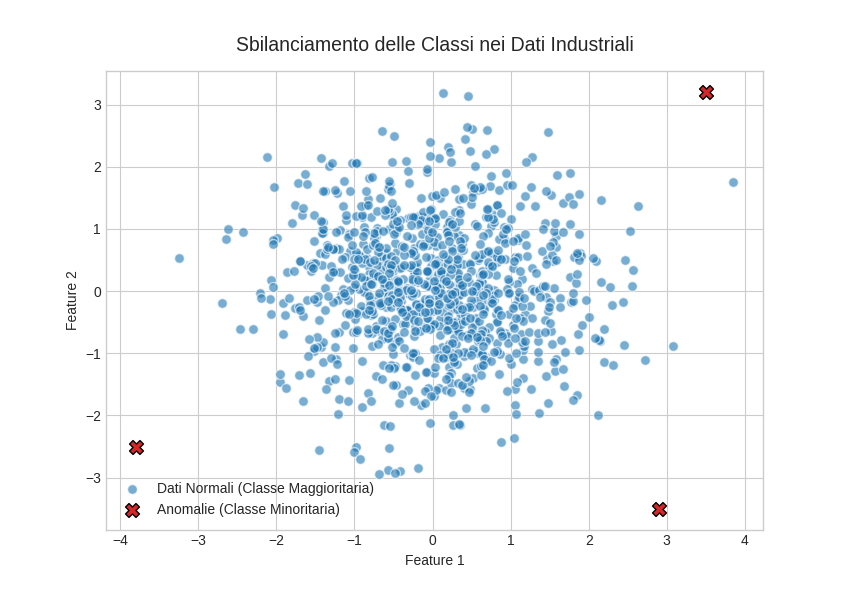
\includegraphics[width=0.8\textwidth]{Sbilaciamento_delle_classi.png}
    \caption{Rappresentazione schematica dello sbilanciamento tra campioni normali ed eventi anomali.}
    \label{fig:sbilanciamento}
\end{figure}

\subsubsection{Variabilità ed eterogeneità delle anomalie}

I difetti possono differire per forma, dimensione, posizione e contrasto rispetto al materiale. Non è quindi realistico assumere di poter rappresentare tutte le loro configurazioni nel training set. Il modello deve distinguere le variazioni compatibili con il prodotto conforme dalle deviazioni significative, generalizzando oltre gli esempi osservati \cite{Aggarwal_et_al._2021,Cui_et_al._2023}.

La Figura~\ref{fig:variabilita_anomalia} illustra, mediante una serie temporale, la distinzione generale tra anomalie puntuali, contestuali e collettive. Nell'ispezione visiva, l'eterogeneità si manifesta invece attraverso alterazioni cromatiche, discontinuità della texture o modifiche della struttura dell'oggetto.

\begin{figure}[htbp]
    \centering
    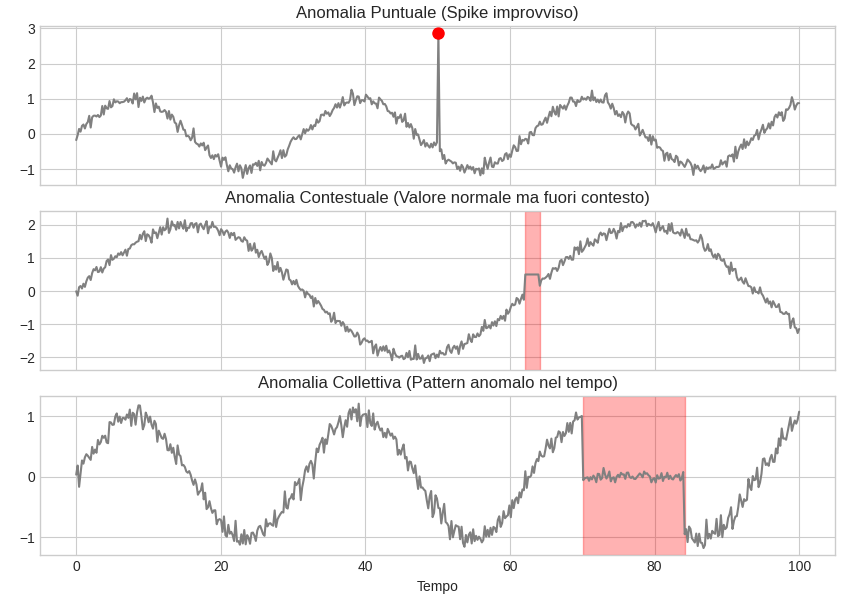
\includegraphics[width=0.8\textwidth]{Variabilita_dell_anomalia.png}
    \caption{Esempio delle tipologie generali di anomalia in una serie temporale: puntuale, contestuale e collettiva.}
    \label{fig:variabilita_anomalia}
\end{figure}

\subsubsection{Dipendenza dal contesto e condizioni di acquisizione}

La normalità dipende dalle condizioni operative. Un valore di temperatura può essere accettabile in una fase produttiva e indicare un guasto in un'altra; analogamente, nell'ispezione visiva, illuminazione, riflessi e variazioni ammesse del materiale possono modificare l'aspetto di un prodotto conforme.

I confini tra variazione normale e difetto possono dunque essere ambigui. Il preprocessing e l'eventuale impiego di informazioni contestuali devono essere progettati in funzione del dominio, per limitare le segnalazioni dovute ai disturbi di acquisizione \cite{Li_et_al._2025,Alzarooni_et_al._2024}. La Figura~\ref{fig:contesto_industriale} esemplifica il ruolo del contesto nella scelta di una soglia di rilevamento.

\begin{figure}[htbp]
    \centering
    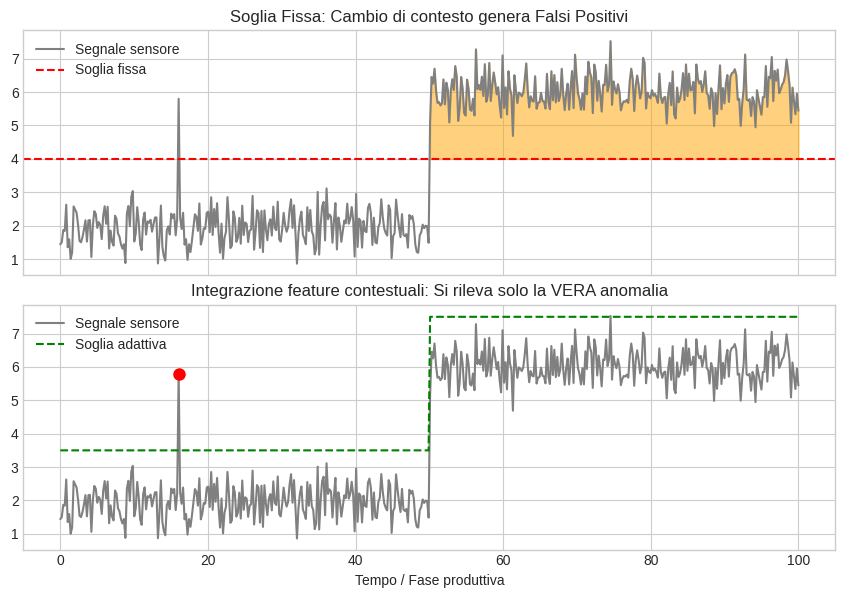
\includegraphics[width=0.8\textwidth]{Soglia_fissa_adattiva.png}
    \caption{Esempio schematico di soglia fissa e soglia adattiva al cambiamento della fase produttiva.}
    \label{fig:contesto_industriale}
\end{figure}

\subsection{Paradigmi di apprendimento e convenzione terminologica}

La disponibilità delle etichette determina quali informazioni possano guidare l'apprendimento. È utile distinguere il paradigma generale dalla granularità delle annotazioni e dalla specifica composizione del training set \cite{Yang_et_al._2021}.

\subsubsection{Apprendimento supervisionato}

Nell'apprendimento supervisionato, ciascun campione è associato a un'etichetta utilizzata durante l'addestramento. Per il rilevamento dei difetti, le etichette possono indicare la conformità dell'intera immagine oppure descrivere le regioni difettose mediante maschere a livello di pixel.

Le annotazioni spaziali richiedono un maggiore lavoro manuale. Le etichette riferite alla sola immagine costituiscono invece una forma di supervisione debole quando l'obiettivo finale è localizzare il difetto. Il vantaggio della supervisione consiste nel fornire esempi espliciti delle anomalie; il limite principale è la necessità di raccogliere campioni sufficientemente rappresentativi \cite{Beitieval_et_al._2024}.

Quando i difetti disponibili sono pochi o poco diversificati, il modello può adattarsi eccessivamente agli esempi osservati e riconoscere con difficoltà anomalie nuove. Questo rischio non implica che tutti i metodi supervisionati falliscano sui difetti sconosciuti, ma rende necessario verificarne la capacità di generalizzazione.

\subsubsection{Apprendimento non supervisionato in senso generale}

Nell'apprendimento non supervisionato non sono disponibili etichette che distinguano i campioni normali da quelli anomali. Molti metodi assumono che le anomalie siano rare e statisticamente distinguibili dalla maggioranza dei dati; il rilevamento dipende quindi dalla rappresentazione adottata e dalla misura di deviazione \cite{Pang_et_al._2021}.

L'assenza di annotazioni riduce il costo di preparazione dei dati, ma non garantisce robustezza alla contaminazione. Se le anomalie influenzano il modello della normalità, possono diventare più difficili da riconoscere. Esistono metodi progettati per affrontare questo problema, la cui efficacia dipende dalle ipotesi e dalle condizioni sperimentali \cite{Lin_et_al._2021}.

\subsubsection{Apprendimento dai soli campioni normali}

Una terza impostazione utilizza un training set composto esclusivamente da campioni noti come normali, senza esempi delle anomalie da rilevare. Nella tassonomia generale dell'anomaly detection, questa impostazione è spesso denominata \textit{semi-supervisionata} \cite{Perez_et_al._2021}. I metodi costruiscono una descrizione della classe normale attraverso confini decisionali, distribuzioni statistiche o rappresentazioni neurali.

Nella letteratura sull'ispezione visiva industriale, lo stesso scenario è comunemente indicato come \textit{unsupervised anomaly detection}, poiché l'apprendimento non richiede esempi annotati dei difetti \cite{Cui_et_al._2023}. Per evitare ambiguità, nel presente elaborato si usa l'espressione \textbf{scenario one-class}: l'adattamento al dominio avviene sui soli campioni normali, mentre le etichette e le maschere del test sono riservate alla valutazione.

Questa convenzione si applica a tutti i modelli selezionati. L'eventuale uso di un backbone pre-addestrato su ImageNet riguarda la provenienza della rappresentazione iniziale e deve essere distinto dalle informazioni impiegate nell'adattamento al dominio industriale.

\section{Il benchmark MVTec AD e le metriche di valutazione}

Un benchmark condiviso permette di confrontare metodi differenti sugli stessi dati e con criteri espliciti. MVTec Anomaly Detection (\textbf{MVTec AD}) è uno dei riferimenti per l'ispezione visiva industriale: comprende campioni normali per l'addestramento e immagini sia normali sia difettose per il test, con annotazioni delle anomalie a livello di pixel \cite{Bergmann_et_al._2019}.

\subsection{Texture e oggetti strutturati}

MVTec AD comprende 5354 immagini ad alta risoluzione, suddivise in quindici categorie:
\begin{itemize}
    \item \textbf{cinque categorie di texture}: tappeto, griglia, pelle, piastrelle e legno;
    \item \textbf{dieci categorie di oggetti}: bottiglia, cavo, capsula, nocciola, dado metallico, pillola, vite, spazzolino, transistor e cerniera.
\end{itemize}

Le texture richiedono soprattutto di riconoscere alterazioni delle regolarità locali; gli oggetti introducono anche vincoli relativi a forma, posizione e composizione delle parti. Il dataset contiene oltre settanta tipologie di difetto, tra cui graffi, contaminazioni, deformazioni e componenti mancanti \cite{Bergmann_et_al._2019}.

La sperimentazione documentata nel presente elaborato riguarda la categoria \texttt{leather}, appartenente alle texture. La descrizione delle altre categorie fornisce il contesto del benchmark, ma non implica che siano incluse negli esperimenti.

\subsection{Estensioni del benchmark}

L'evoluzione dei metodi ha motivato la costruzione di dataset complementari. \textbf{MVTec LOCO AD} (\textit{Logical Constraints Anomaly Detection}) comprende 3644 immagini e considera sia anomalie strutturali sia violazioni di vincoli logici, come componenti corretti collocati nella posizione sbagliata \cite{MVTech_LOCO_AD}.

\textbf{MVTec AD 2} amplia invece la varietà degli scenari industriali con oltre 8000 immagini ad alta risoluzione. Include oggetti sovrapposti, materiali trasparenti o semitrasparenti, variazioni di acquisizione e difetti di piccole dimensioni rispetto all'immagine \cite{Steger_et_al._2026}. Queste condizioni mettono alla prova capacità che possono essere poco sollecitate dai benchmark precedenti.

I dataset citati in questa sezione inquadrano le sfide della ricerca; non costituiscono dati sperimentali del confronto descritto nel Capitolo~\ref{chap:implementazione}.

\subsection{Criteri di valutazione}

Il confronto distingue la discriminazione dell'intera immagine dalla localizzazione del difetto. Le metriche basate su curve valutano il comportamento al variare della soglia, mentre quelle calcolate su una singola segmentazione dipendono dalla soglia scelta \cite{Zheng_et_al._2022}.

\subsubsection{AUROC a livello di immagine}

La curva ROC rappresenta il tasso di veri positivi (\textit{true positive rate}, TPR) in funzione del tasso di falsi positivi (\textit{false positive rate}, FPR):
\[
    \mathrm{TPR}=\frac{\mathrm{TP}}{\mathrm{TP}+\mathrm{FN}},
    \qquad
    \mathrm{FPR}=\frac{\mathrm{FP}}{\mathrm{FP}+\mathrm{TN}}.
\]
Le anomalie costituiscono la classe positiva. L'area sotto la curva, denominata AUROC, misura la capacità dei punteggi di discriminare campioni normali e difettosi al variare della soglia.

A livello di immagine, il calcolo richiede un punteggio globale per ciascun campione. Nel protocollo adottato, tale punteggio è il massimo della mappa di anomalia. Un'AUROC elevata indica una buona separazione dei campioni nel test esaminato, ma non determina una soglia operativa né garantisce la stessa prestazione su dati futuri.

\subsubsection{AUROC a livello di pixel}

L'AUROC a livello di pixel confronta i punteggi della mappa con le annotazioni della ground truth. La metrica valuta l'ordinamento dei pixel normali e anomali, ma non descrive direttamente la precisione dei contorni o la copertura di ciascun difetto.

Poiché TPR e FPR sono normalizzati sulle rispettive classi, il predominio numerico dei pixel normali non equivale, da solo, a un aumento dell'AUROC. Rimangono però limiti interpretativi: il raggruppamento dei pixel attribuisce maggiore peso alle anomalie estese e l'integrazione sull'intera curva può nascondere un comportamento insoddisfacente ai bassi FPR rilevanti per l'ispezione industriale \cite{Bertoldo_et_al._2024}. Per questo l'AUROC deve essere affiancata da misure complementari e dall'esame delle mappe.

\subsubsection{PRO e AU-PRO}

Il \textit{Per-Region Overlap} (PRO) misura, a una data soglia, la frazione di pixel rilevati all'interno di ciascuna regione anomala connessa e ne calcola la media. Le regioni ricevono così lo stesso peso, indipendentemente dalla loro area. I falsi positivi esterni ai difetti sono considerati attraverso il FPR associato alla soglia \cite{Zheng_et_al._2022}.

L'AU-PRO integra il PRO in funzione del FPR entro un intervallo dichiarato. Nel protocollo del progetto, il limite superiore è 0,3 e l'area è normalizzata rispetto a tale intervallo. L'indicazione del limite e della normalizzazione è necessaria per interpretare e confrontare i valori.

\subsubsection{Metriche a soglia e analisi qualitativa}

Il punteggio F1 combina precisione e richiamo:
\[
    \mathrm{F1}=
    \frac{2\,\mathrm{precision}\,\mathrm{recall}}
    {\mathrm{precision}+\mathrm{recall}}.
\]
Nei risultati del progetto, il massimo F1 è ottenuto scegliendo la soglia sul test set e costituisce quindi una misura retrospettiva \textit{oracle}. Non rappresenta una prestazione operativa con soglia selezionata su dati indipendenti. Il calcolo pixel-level è inoltre approssimato mediante campionamento spaziale con stride 4 e una griglia di 500 soglie.

L'analisi qualitativa completa questi indicatori confrontando immagini, maschere e mappe. Permette di osservare localizzazioni incomplete, risposte diffuse e attivazioni su regioni normali, distinguendo i comportamenti visibili dalle ipotesi sulle loro cause.

\section{Obiettivi e struttura dell'elaborato}

Il lavoro analizza in modo comparativo quattro pipeline di rilevamento delle anomalie visive industriali: \textbf{CCW-SSIM}, \textbf{PaDiM}, \textbf{RD4AD} e \textbf{FastFlow}. I modelli rappresentano approcci differenti alla costruzione della normalità: ricostruzione dell'immagine, modellazione statistica delle feature, distillazione della conoscenza e flussi di normalizzazione.

Il perimetro sperimentale è circoscritto alla categoria \texttt{leather} di MVTec AD, assunta come unico caso di studio. Il confronto riguarda le implementazioni e le configurazioni adottate, con dati e protocollo di valutazione condivisi. Le differenze di risoluzione, pre-addestramento e regime di apprendimento sono parte dell'interpretazione dei risultati; il confronto non isola l'effetto della sola famiglia metodologica.

Gli obiettivi sono valutare la discriminazione delle immagini e la localizzazione dei difetti, esaminare qualitativamente le mappe e discutere i costi osservati e i limiti delle pipeline. L'estensione ad altre categorie e le prove dedicate a colore, illuminazione o fine-tuning costituiscono possibili approfondimenti, da distinguere dagli esperimenti già documentati.

Il Capitolo~\ref{chap:stato-arte} presenta lo stato dell'arte e i principi dei metodi selezionati. Il Capitolo~\ref{chap:implementazione} descrive le implementazioni e il protocollo comune. Il Capitolo~\ref{chap:risultati} analizza quantitativamente e qualitativamente i risultati, mettendoli in relazione con le fonti di riferimento. Il Capitolo~\ref{chap:conclusioni} sintetizza quanto emerso nel caso di studio e discute i limiti della ricerca e le possibili estensioni.

\chapter{Stato dell'arte}
\label{chap:stato-arte}

Definiti il problema e i criteri di valutazione, occorre esaminare i metodi con cui apprendere la normalità visiva e riconoscerne le deviazioni. Nell'ispezione industriale, l'obiettivo è riconoscere difetti anche quando non sono disponibili esempi rappresentativi di tutte le anomalie possibili \cite{Yang_et_al._2021,Cui_et_al._2023}.

Le applicazioni comprendono il controllo di qualità, l'analisi di immagini mediche e il rilevamento di eventi nei video. Questi ambiti condividono il problema della scarsità delle anomalie, ma differiscono per dati, vincoli e modalità di valutazione. La rassegna seguente privilegia l'ispezione di immagini industriali, che costituisce il dominio della sperimentazione.

\section{Criteri di classificazione dei metodi}

La letteratura può essere organizzata secondo tre assi distinti:
\begin{itemize}
    \item \textbf{dominio dei dati}: immagini, video o rappresentazioni tridimensionali;
    \item \textbf{informazioni disponibili durante l'apprendimento}: campioni normali, esempi di anomalie e annotazioni di diversa granularità;
    \item \textbf{meccanismo di rilevamento}: ricostruzione, distanze nello spazio delle feature, stima di densità o discriminazione appresa.
\end{itemize}

Questi criteri non sono intercambiabili. Un'architettura non determina da sola il paradigma di supervisione e uno stesso metodo può combinare più meccanismi. La tassonomia serve quindi a chiarire il ruolo delle componenti, evitando di considerare le famiglie come categorie necessariamente disgiunte \cite{Cui_et_al._2023}.

\subsection{Granularità dell'output e supervisione}

Il rilevamento a livello di immagine produce un punteggio per l'intera immagine; la localizzazione a livello di pixel produce una mappa spaziale. Una segmentazione binaria può essere ottenuta applicando una soglia alla mappa. L'esistenza di un output spaziale non implica che il modello sia stato addestrato usando maschere dei difetti.

Come definito nel Capitolo~\ref{chap:introduzione}, il progetto adotta uno scenario \textit{one-class}: i campioni industriali utilizzati per l'adattamento sono tutti normali. Le maschere del test sono impiegate nella valutazione. I modelli possono comunque utilizzare rappresentazioni pre-addestrate su altri dataset. Altri metodi one-class introducono anomalie sintetiche per costruire compiti auto-supervisionati; questa procedura non è utilizzata dalle quattro pipeline sperimentate.

La Tabella~\ref{tab:taxonomy} distingue le principali informazioni che possono guidare l'apprendimento.
\begin{table}[htbp]
    \centering
    \small
    \caption{Informazioni di addestramento e ruolo delle annotazioni nell'ispezione visiva.}
    \label{tab:taxonomy}
    \begin{tabularx}{\textwidth}{@{}P{0.24\textwidth}YY@{}}
        \hline
        \textbf{Impostazione} & \textbf{Dati disponibili} & \textbf{Informazione utilizzata} \\
        \hline
        Supervisionata & Campioni normali e difettosi & Etichette di classe o maschere dei difetti \\
        Debolmente supervisionata & Annotazioni meno dettagliate dell'output richiesto & Ad esempio, etichette di immagine per localizzare un difetto \\
        One-class & Campioni industriali noti come normali & Modellazione della normalità senza esempi reali dei difetti \\
        Non supervisionata in senso generale & Campioni non etichettati, eventualmente contaminati & Regolarità statistiche dei dati e ipotesi sulle anomalie \\
        \hline
    \end{tabularx}
\end{table}

\section{Metodi basati su descrittori manuali}

Prima della diffusione delle reti profonde, molte pipeline combinavano descrittori progettati manualmente (\textit{handcrafted features}) con classificatori o stimatori statistici \cite{Yang_et_al._2021}. L'efficacia dipendeva dalla capacità dei descrittori di rappresentare le variazioni rilevanti per il dominio.

Tra gli strumenti utilizzati si distinguono:
\begin{itemize}
    \item \textbf{descrittori locali}: SIFT (\textit{Scale-Invariant Feature Transform}) per punti di interesse invarianti alla scala, HOG (\textit{Histograms of Oriented Gradients}) per orientazioni dei gradienti e LBP (\textit{Local Binary Patterns}) per regolarità locali della texture \cite{Yang_et_al._2021,Cui_et_al._2023};
    \item \textbf{filtri e trasformate}: operatori di gradiente, rilevamento dei bordi, filtri di Gabor e trasformate di Fourier o wavelet per descrivere frequenze, orientazioni e discontinuità \cite{Cui_et_al._2023}.
\end{itemize}

Le rappresentazioni potevano essere utilizzate da tre principali classi di metodi decisionali:
\begin{enumerate}
    \item \textbf{Stima di densità}. Modelli a mistura gaussiana (GMM) e stimatori di densità basati su kernel (KDE) descrivono la distribuzione dei campioni. Una densità bassa rispetto al modello può segnalare un'anomalia.
    \item \textbf{Classificazione one-class}. One-Class SVM (OCSVM) e Support Vector Data Description (SVDD) costruiscono un confine attorno ai campioni normali nello spazio delle feature.
    \item \textbf{Modelli spaziali e temporali}. I campi aleatori di Markov (MRF) e altri modelli contestuali considerano dipendenze tra osservazioni. Nell'analisi video possono essere affiancati da descrittori del movimento \cite{Tran_et_al._2022}.
\end{enumerate}

L'alta dimensionalità e le variazioni di illuminazione o texture possono rendere difficile la scelta delle feature. Inoltre, l'estrazione e la decisione sono spesso ottimizzate separatamente. Questi limiti hanno motivato lo sviluppo di rappresentazioni apprese; i metodi tradizionali rimangono tuttavia utili quando i dati sono limitati o i vincoli computazionali favoriscono soluzioni semplici \cite{Yang_et_al._2021}.

\section{Famiglie di metodi basati sul deep learning}

Le reti profonde permettono di apprendere descrittori multilivello e di combinare informazione locale e rappresentazioni più astratte. Alcuni metodi addestrano una rete sul dominio industriale; altri utilizzano un estrattore pre-addestrato e stimano soltanto un modello delle feature normali.

Le sezioni seguenti presentano cinque famiglie utili a inquadrare i quattro modelli selezionati. La sintesi evidenzia sia i principi condivisi sia le differenze che dovranno essere considerate nel confronto sperimentale \cite{Cui_et_al._2023}.

\subsection{Metodi basati sulla ricostruzione}

I metodi ricostruttivi apprendono a riprodurre immagini normali attraverso una rappresentazione latente. L'ipotesi è che i difetti, non osservati durante l'addestramento, siano ricostruiti meno fedelmente e producano una discrepanza maggiore \cite{Yang_et_al._2021}. Questa proprietà deve essere verificata: una rete sufficientemente flessibile può ricostruire anche anomalie.

Negli autoencoder, l'encoder comprime l'input e il decoder ne genera una ricostruzione. La funzione obiettivo può misurare differenze tra pixel o utilizzare indici strutturali. Una possibile combinazione è
\[
    \mathcal{L}_{\mathrm{rec}}(x,\widehat{x}) =
    (1-\alpha)\lVert x-\widehat{x}\rVert_2
    +\alpha\bigl(1-\mathrm{SSIM}(x,\widehat{x})\bigr),
    \qquad 0\leq\alpha\leq1.
\]
La formula illustra un criterio ricostruttivo e non una perdita universale della famiglia. Il calcolo di una mappa locale richiede inoltre di specificare come le discrepanze siano valutate nello spazio.

Nei modelli generativi come AnoGAN, la ricerca della ricostruzione più vicina può richiedere un'ottimizzazione del vettore latente. Il criterio combina un residuo dell'immagine con una discrepanza tra feature del discriminatore:
\[
    \mathcal{L}_{\mathrm{AnoGAN}}(z)=
    (1-\lambda)\lVert x-G(z)\rVert_1
    +\lambda\lVert D_{\mathrm{feat}}(x)
    -D_{\mathrm{feat}}(G(z))\rVert_1.
\]
Qui $G$ è il generatore e $D_{\mathrm{feat}}$ indica una rappresentazione intermedia del discriminatore \cite{Schlegl_et_al._2017}.

Tra gli sviluppi della famiglia, CAVGA introduce vincoli di attenzione, mentre DFR (\textit{Deep Feature Reconstruction}) ricostruisce rappresentazioni estratte da una rete pre-addestrata anziché direttamente i pixel. La ricostruzione può quindi operare in spazi differenti e sovrapporsi ad altri approcci della tassonomia \cite{Cui_et_al._2023}.

CCW-SSIM, selezionato per il progetto, appartiene a questa famiglia: combina la ricostruzione mediante autoencoder con una valutazione della discrepanza strutturale e cromatica \cite{Berasi_2023}. Il suo interesse per il confronto consiste nell'apprendere direttamente dai campioni industriali senza utilizzare un backbone ImageNet.

\subsection{Metodi basati sulle rappresentazioni}

Questi metodi descrivono i campioni mediante vettori di caratteristiche, indicati come \textit{feature}, spesso estratte da reti pre-addestrate. Il punteggio di anomalia deriva dal confronto con feature normali conservate in memoria oppure con statistiche stimate su di esse \cite{Cui_et_al._2023}.

La famiglia comprende approcci con estrattore congelato e varianti che adattano le rappresentazioni al dominio. Non è quindi corretto attribuire a tutti l'assenza di addestramento neurale.

PaDiM (\textit{Patch Distribution Modeling}) stima una gaussiana multivariata per ciascuna posizione spaziale. Il punteggio locale usa la distanza di Mahalanobis:
\[
    D_M(z)=\sqrt{(z-\mu)^{\mathrm{T}}\Sigma^{-1}(z-\mu)},
\]
dove $z$ è il vettore di feature, $\mu$ la media locale e $\Sigma$ la covarianza stimata sui campioni normali. La distanza considera variabilità e correlazioni tra componenti, a differenza della distanza euclidea \cite{Defard_et_al._2021}.

Altri esempi sono:
\begin{itemize}
    \item \textbf{SPADE}: confronta feature multiscala attraverso ricerche dei vicini più prossimi; la consultazione dei campioni di riferimento contribuisce al costo di inferenza \cite{Yang_et_al._2021};
    \item \textbf{PatchCore}: conserva feature normali in una \textit{memory bank}, riducendola mediante selezione di un sottoinsieme rappresentativo (\textit{coreset}) \cite{Roth_et_al._2022};
    \item \textbf{CFA} (\textit{Coupled-hypersphere-based Feature Adaptation}): adatta le feature al dominio attraverso vincoli geometrici \cite{Cui_et_al._2023}.
\end{itemize}

Il vantaggio dell'estrattore pre-addestrato è la disponibilità di rappresentazioni già strutturate. Il limite è la possibile distanza tra il dominio del pre-addestramento e le caratteristiche dei materiali industriali. Memoria, costo di adattamento e inferenza dipendono poi dalla specifica modalità di confronto.

\subsection{Metodi basati sulla distillazione Teacher--Student}

La distillazione utilizza una rete \textit{Teacher} per fornire rappresentazioni di riferimento e una rete \textit{Student} addestrata a riprodurle sui campioni normali. In inferenza, la discrepanza tra le rappresentazioni può segnalare una deviazione dalla normalità \cite{Cui_et_al._2023}.

Indicando con $f_T^k(x)$ e $f_S^k(x)$ le feature corrispondenti al livello $k$, una forma generale dell'obiettivo è
\[
    \mathcal{L}_{\mathrm{dist}}=
    \sum_k d\bigl(f_T^k(x),f_S^k(x)\bigr),
\]
dove la distanza $d$ e la modalità di aggregazione dipendono dal metodo. Il punteggio spaziale in inferenza può utilizzare un'aggregazione diversa da quella impiegata nell'addestramento.

RD4AD adotta la \textit{reverse distillation}: lo Student è un decoder che riceve una rappresentazione compressa delle feature del Teacher e tenta di ricostruirle. Un \textit{One-Class Bottleneck Embedding} (OCBE) aggrega le informazioni multiscala. La struttura asimmetrica mira a limitare il trasferimento indiscriminato delle informazioni anomale allo Student \cite{Deng_et_al._2022}.

Il metodo ricostruisce dunque feature anziché immagini. Questa relazione con gli approcci ricostruttivi chiarisce perché la tassonomia sia uno strumento descrittivo e non una separazione rigida. Nel progetto, RD4AD permette di confrontare la ricostruzione distillata delle feature con la modellazione statistica di PaDiM.

\subsection{Metodi basati sui flussi di normalizzazione}

I \textit{normalizing flows} apprendono trasformazioni invertibili tra una distribuzione complessa e una distribuzione di riferimento trattabile. Nell'ispezione visiva possono operare sulle feature estratte da un backbone \cite{Cui_et_al._2023}.

Se $z=f_\theta(x)$ è una trasformazione invertibile, il cambio di variabile fornisce
\[
    p_X(x)=p_Z(f_\theta(x))
    \left|\det\frac{\partial f_\theta(x)}{\partial x}\right|,
\]
e quindi
\[
    \log p_X(x)=\log p_Z(f_\theta(x))
    +\log\left|\det\frac{\partial f_\theta(x)}{\partial x}\right|.
\]
La distribuzione $p_Z$ è spesso una normale standard. L'addestramento massimizza la log-verosimiglianza dei campioni normali; il punteggio di anomalia in inferenza deve essere definito in modo coerente con la specifica implementazione. Una densità bassa non equivale direttamente a una probabilità calibrata di difetto.

Tra gli esempi della famiglia:
\begin{itemize}
    \item \textbf{DifferNet} applica flussi alle feature per il rilevamento a livello di immagine;
    \item \textbf{CFLOW-AD} impiega flussi condizionali per la localizzazione;
    \item \textbf{FastFlow} utilizza trasformazioni bidimensionali sulle mappe di feature, mantenendo la struttura spaziale utile alla localizzazione \cite{Yu_et_al._2021}.
\end{itemize}

FastFlow è il rappresentante selezionato nel progetto. La formulazione generale permette estrattori differenti, ma il confronto documentato utilizza un backbone convoluzionale congelato. Il Capitolo~\ref{chap:implementazione} distingue la funzione obiettivo del flusso dalla costruzione effettiva della mappa di anomalia.

\subsection{Metodi basati sulla sintesi di anomalie}

Un'ulteriore famiglia genera alterazioni artificiali dei campioni normali per costruire un segnale di apprendimento. L'assenza di esempi reali dei difetti non impedisce così l'impiego di etichette sintetiche per compiti di classificazione o segmentazione \cite{Cui_et_al._2023}.

Per la segmentazione, una possibile componente dell'obiettivo è l'entropia incrociata binaria:
\[
    \ell(y,p)=-\bigl[y\log p+(1-y)\log(1-p)\bigr],
\]
dove $y$ indica se il pixel appartenga alla regione alterata e $p$ è la previsione della rete. La funzione è calcolata sui pixel e aggregata secondo il metodo; possono essere presenti altre componenti di perdita.

Esempi di questa famiglia sono:
\begin{itemize}
    \item \textbf{CutPaste}: ritaglia regioni di un'immagine normale, le modifica e le reinserisce per costruire un compito di riconoscimento delle alterazioni;
    \item \textbf{DRAEM}: combina una rete ricostruttiva con una rete discriminativa per apprendere la localizzazione di anomalie simulate \cite{Zavrtanik_et_al._2021};
    \item \textbf{NSA} (\textit{Natural Synthetic Anomalies}): fonde patch provenienti da altre immagini attraverso tecniche di \textit{Poisson image editing} \cite{Cui_et_al._2023}.
\end{itemize}

La difficoltà principale riguarda la relazione tra difetti artificiali e reali: un modello può apprendere caratteristiche della procedura di sintesi che non siano rappresentative delle anomalie industriali. Questi metodi completano il quadro della letteratura, ma non sono inclusi nel confronto sperimentale.

\subsection{Sintesi e collegamento con i modelli selezionati}

La Tabella~\ref{tab:metodi_ad} riassume i principi e i limiti delle famiglie discusse. Le indicazioni sono qualitative: non costituiscono una graduatoria di accuratezza, memoria o velocità indipendente dall'implementazione.

\begin{table}[htbp]
    \centering
    \small
    \caption{Principi e principali limiti delle famiglie di metodi.}
    \label{tab:metodi_ad}
    \renewcommand{\arraystretch}{1.15}
    \begin{tabularx}{\textwidth}{@{}P{0.21\textwidth}YY@{}}
        \hline
        \textbf{Famiglia} & \textbf{Principio ed esempi} & \textbf{Limiti da considerare} \\
        \hline
        Descrittori manuali & Feature progettate e modelli statistici; SIFT, GMM, OCSVM & Scelta delle feature e sensibilità alle condizioni di acquisizione \\
        Ricostruzione & Discrepanza tra input e ricostruzione; autoencoder, CCW-SSIM & Possibile ricostruzione anche dei difetti \\
        Rappresentazioni & Confronto con feature normali o statistiche; PaDiM, PatchCore & Dipendenza dall'estrattore e costo di memoria \\
        Distillazione & Discrepanza Teacher--Student; RD4AD & Dipendenza dalle feature e dalla capacità dello Student \\
        Flussi di normalizzazione & Trasformazione invertibile delle feature; FastFlow & Scelte dell'estrattore, dei flussi e del punteggio \\
        Sintesi di anomalie & Apprendimento da alterazioni artificiali; CutPaste, DRAEM & Corrispondenza tra anomalie sintetiche e reali \\
        \hline
    \end{tabularx}
\end{table}

I quattro modelli selezionati condividono l'adattamento sui soli campioni normali, ma differiscono nello spazio in cui descrivono la normalità e nel criterio con cui ne misurano le deviazioni. Queste differenze motivano un confronto che consideri insieme discriminazione globale, localizzazione e comportamento delle mappe.

\section{Sfide aperte e limiti di applicazione}

Le prestazioni su un benchmark non esauriscono i requisiti di un sistema industriale. Il trasferimento richiede di considerare acquisizione dei dati, cambiamenti del dominio e risorse disponibili \cite{Alzarooni_et_al._2024,Li_et_al._2025}. Le questioni seguenti costituiscono un quadro interpretativo, da distinguere dalle proprietà effettivamente misurate nel progetto.

\subsection{Differenze di dominio e adattamento delle feature}

I backbone pre-addestrati su dataset generici, come ImageNet, rendono disponibili rappresentazioni senza richiedere di apprendere da zero l'intero estrattore \cite{Roth_et_al._2022}. Tuttavia, le caratteristiche utili alla classificazione di immagini naturali possono non descrivere in modo ottimale microstrutture e difetti industriali.

L'adattamento delle feature può ridurre questa distanza, ma richiede di verificare che la rappresentazione conservi la capacità di distinguere anomalie non osservate \cite{Li_et_al._2025}. Nel progetto, PaDiM, RD4AD e FastFlow condividono un backbone congelato; CCW-SSIM apprende invece dai soli campioni industriali. Questa differenza deve essere considerata nell'interpretazione dei risultati.

\subsection{Scalabilità computazionale ed edge computing}

L'esecuzione su dispositivi periferici può imporre vincoli di memoria, latenza ed energia, discussi sia per l'ispezione visiva industriale sia, più in generale, per le reti IoT \cite{Li_et_al._2025,Morshedi_et_al._2025}. Il costo dipende dall'estrattore, dalla risoluzione, dai componenti addestrabili e dal trattamento delle mappe.

Nei metodi con memory bank, la selezione di un coreset limita la quantità di feature conservate, ma la consultazione dei riferimenti rimane parte dell'inferenza \cite{Roth_et_al._2022}. Nei modelli neurali, il costo dell'addestramento deve essere distinto dal tempo di predizione. Per questo, un tempo di addestramento basso non dimostra da solo l'idoneità a operare in tempo reale.

\subsection{Cambiamenti del dominio e apprendimento continuo}

Molti esperimenti assumono che le condizioni di addestramento e test siano stabili. Nelle applicazioni possono invece cambiare illuminazione, strumenti di acquisizione o caratteristiche del prodotto. Il modello appreso può così perdere validità e produrre più falsi allarmi.

La \textit{continual anomaly detection} studia aggiornamenti incrementali della normalità, affrontando il rischio di dimenticare informazioni precedenti (\textit{catastrophic forgetting}) o di incorporare anomalie non riconosciute. Una rassegna recente di questi temi è disponibile come preprint, non sottoposto a peer review \cite{Faber_et_al._2026}. La presenza di anomalie mai viste va distinta da questi cambiamenti della normalità: sono due aspetti diversi della generalizzazione.

\subsection{Approcci zero-shot e foundation models}

Quando è difficile raccogliere campioni normali specifici del prodotto, gli approcci \textit{zero-shot} cercano di rilevare anomalie senza adattamento sul dominio di destinazione. Modelli visivo-linguistici e altri foundation models possono fornire rappresentazioni e indicazioni semantiche mediante prompt.

Il framework DCS esplora, ad esempio, l'integrazione di DINO, CLIP e SAM per il rilevamento e la segmentazione \cite{Wan_et_al._2026}. Queste possibilità ampliano il quadro della ricerca, ma richiedono valutazioni specifiche della precisione locale e dei costi. Non fanno parte dei metodi sperimentati nel presente lavoro.

La rassegna conduce quindi a una domanda circoscritta: come si comportano quattro diverse pipeline one-class quando sono adattate e valutate sullo stesso caso di studio? Il capitolo seguente documenta le configurazioni necessarie a rendere esplicite le condizioni di tale confronto.

\chapter[Modelli selezionati e implementazione]{Modelli selezionati e implementazione sperimentale}
\label{chap:implementazione}

Le famiglie presentate nello stato dell'arte descrivono modi differenti di apprendere la normalità e riconoscere le anomalie. Per confrontarle sul caso di studio occorre tradurre questi principi in pipeline concrete, definendo come vengono elaborate le immagini, quali componenti apprendono dai campioni normali e come viene costruita la mappa di anomalia. Il capitolo sviluppa questo passaggio attraverso i quattro modelli selezionati: \textbf{CCW-SSIM}, \textbf{PaDiM}, \textbf{RD4AD} e \textbf{FastFlow}.

Il punto di partenza comune è costituito dalle immagini di \textbf{MVTec AD}, impiegate per l'adattamento al dominio industriale e per il test. Le rappresentazioni iniziali hanno invece una provenienza diversa: PaDiM, RD4AD e FastFlow utilizzano backbone con pesi pre-addestrati su \textbf{ImageNet}, mentre CCW-SSIM apprende da zero sui campioni normali del materiale. Questa differenza aiuta a comprendere sia le procedure di apprendimento sia i costi delle configurazioni adottate.

\section{Criteri di selezione e ruolo dei modelli}
\label{sec:cap3-criteri}

La scelta dei modelli permette di esaminare quattro famiglie metodologiche discusse nel Capitolo~\ref{chap:stato-arte}:
\begin{itemize}
    \item \textbf{CCW-SSIM} \cite{Berasi_2023} appartiene ai metodi basati sulla ricostruzione. Un autoencoder apprende a riprodurre i campioni normali e la discrepanza tra immagine originale e ricostruita è valutata considerando congiuntamente struttura e colore;
    \item \textbf{PaDiM} \cite{Defard_et_al._2021} è un metodo basato sulla rappresentazione. Le feature estratte da una rete pre-addestrata sono modellate, per ciascuna posizione spaziale, mediante una distribuzione gaussiana multivariata;
    \item \textbf{RD4AD} \cite{Deng_et_al._2022} adotta la \textit{Reverse Distillation}. Un encoder \textit{Teacher} congelato fornisce le rappresentazioni di riferimento, mentre un collo di bottiglia e un decoder \textit{Student} apprendono a ricostruirle sui soli campioni normali;
    \item \textbf{FastFlow} \cite{Yu_et_al._2021} impiega flussi di normalizzazione bidimensionali. Trasformazioni invertibili apprendono la distribuzione delle feature normali preservandone l'organizzazione spaziale.
\end{itemize}

I quattro approcci rappresentano pertanto modalità differenti di costruire un modello della normalità: ricostruzione dell'immagine, stima statistica locale delle feature, ricostruzione distillata delle feature e stima esplicita della loro densità.

L'implementazione adotta lo scenario \textit{one-class} definito nel Capitolo~\ref{chap:introduzione}: la fase di adattamento utilizza esclusivamente immagini prive di difetti. Le immagini normali e anomale della partizione di test sono elaborate nella successiva fase di inferenza; le etichette e le maschere dei difetti sono utilizzate per la valutazione, secondo il protocollo illustrato nel capitolo dedicato ai risultati.

All'interno di questo scenario, l'apprendimento assume forme diverse. CCW-SSIM, RD4AD e FastFlow ottimizzano parametri neurali; PaDiM stima le statistiche gaussiane delle feature normali mantenendo congelato il backbone. Il confronto comprende quindi sia modelli con addestramento iterativo sia un approccio di adattamento statistico. Prima di descriverli singolarmente, è utile chiarire i dati e l'organizzazione sperimentale che condividono.

\section{Ambiente e protocollo implementativo comune}
\label{sec:cap3-ambiente}

\subsection{Dataset MVTec AD e categoria leather}

MVTec AD \cite{Bergmann_et_al._2019} raccoglie immagini industriali ad alta risoluzione, organizzate in categorie di oggetti e texture. Il repository conserva le quindici categorie del dataset; le configurazioni e i manifesti verificabili per i quattro modelli fanno tuttavia riferimento alla categoria \texttt{leather}.

Per tale categoria, la partizione \texttt{train/good} contiene 245 immagini normali. La partizione di test contiene 124 immagini: 32 normali e 92 appartenenti alle tipologie di difetto \texttt{color}, \texttt{cut}, \texttt{fold}, \texttt{glue} e \texttt{poke}. Per le immagini difettose sono disponibili 92 maschere nella directory \texttt{ground\_truth}. La medesima organizzazione dei dati è condivisa da tutte le implementazioni.

\subsection{Organizzazione del repository e pipeline di esecuzione}

Il repository comprende una directory per ciascun modello: \texttt{CCW-SSIM}, \texttt{PaDiM}, \texttt{RD4AD} e \texttt{FastFlow}. Ogni directory contiene un punto di ingresso \texttt{Main.py}, una configurazione dedicata e i moduli per caricamento dei dati, costruzione del modello, adattamento e inferenza. Il notebook \texttt{pipeline\_tesi.ipynb} coordina l'esecuzione.

Il dataset è conservato nella directory centrale \texttt{MVTec\_Data} condivisa tra le singole directory locali dei modelli. L'esecuzione comune è articolata nelle seguenti fasi:
\begin{itemize}
    \item adattamento del modello sui campioni normali presenti in \texttt{train/good};
    \item caricamento del checkpoint o delle statistiche apprese;
    \item inferenza sulle immagini della partizione di test;
    \item salvataggio delle mappe di anomalia e dei metadati di esecuzione.
\end{itemize}

Il modulo \texttt{experiment\_protocol.py} registra manifesti e impronte dei file impiegati, rendendo esplicite la configurazione e la provenienza degli artefatti.

\subsection{Ambiente software e hardware}

Gli ambienti registrati nei manifesti del progetto utilizzano Linux su architettura \texttt{x86\_64} e Python~3.11.15. CCW-SSIM è implementato con TensorFlow~2.15 e le API Keras, mentre PaDiM, RD4AD e FastFlow utilizzano PyTorch~2.13.0 e Torchvision~0.28. Le configurazioni rilevate sono riassunte nella Tabella~\ref{tab:cap3-ambienti}.

\begin{table}[htbp]
    \centering
    \small
    \begin{tabularx}{\textwidth}{|P{2.3cm}|Y|Y|}
        \hline
        \textbf{Modello} & \textbf{Framework} & \textbf{Supporto GPU registrato} \\
        \hline
        CCW-SSIM & TensorFlow 2.15, API Keras & CUDA 12.2, cuDNN 8 \\
        \hline
        PaDiM & PyTorch 2.13.0, Torchvision 0.28 & CUDA 13.0 \\
        \hline
        RD4AD & PyTorch 2.13.0, Torchvision 0.28 & CUDA 13.0 \\
        \hline
        FastFlow & PyTorch 2.13.0, Torchvision 0.28 & CUDA 13.0 \\
        \hline
    \end{tabularx}
    \caption{Ambienti software registrati per le implementazioni.}
    \label{tab:cap3-ambienti}
\end{table}

La gestione dell'ambiente radice è definita dai file \texttt{pyproject.toml} e \texttt{uv.lock}. I manifesti indicano l'impiego di una GPU NVIDIA GeForce RTX~4070~Ti.

\subsection{Gestione di configurazioni, checkpoint e artefatti}

Tutte le pipeline fissano il seme pseudo-casuale a 1024. I parametri sono mantenuti nei rispettivi file di configurazione, mentre i pesi o le statistiche apprese sono salvati in formati specifici per il framework: file HDF5 per CCW-SSIM, file \texttt{pickle} per PaDiM e file PTH per RD4AD e FastFlow.

Le mappe di anomalia sono memorizzate come immagini TIFF in virgola mobile a 32 bit, senza quantizzazione preventiva. A ogni esecuzione sono inoltre associati un manifesto JSON e, per i modelli ottimizzati iterativamente, la cronologia di addestramento in formato CSV. Le mappe costituiscono il collegamento tra implementazione e valutazione: da esse saranno ricavati i punteggi delle immagini e le misure di localizzazione discusse nel Capitolo~\ref{chap:risultati}.

\section{CCW-SSIM}
\label{sec:cap3-ccw}

\subsection{Ricostruzione e confronto percettivo}

CCW-SSIM è un metodo basato sulla ricostruzione \cite{Berasi_2023}. Un autoencoder convoluzionale comprime l'immagine in una rappresentazione latente e la ricostruisce. L'addestramento sui soli campioni normali induce la rete a rappresentare regolarità cromatiche e strutturali proprie del dominio osservato.

Indicando con $x$ l'immagine di ingresso e con $g_{\theta}$ l'autoencoder, la ricostruzione è
\begin{equation}
    \widehat{x} = g_{\theta}(x).
\end{equation}
Per valutare la ricostruzione, il modello combina una misura strutturale, derivata dalla CW-SSIM, con una componente cromatica percettiva. Il confronto richiede quindi una trasformazione dell’immagine che separi luminanza e crominanza.

La trasformazione S-CIELAB converte l'immagine RGB nello spazio XYZ, separa l'informazione in canali opponenti e applica filtri spaziali differenti alle componenti di luminanza e crominanza. Dopo la riconversione in CIELAB si ottengono i canali $L^*$, $a^*$ e $b^*$. Il filtraggio tiene conto della diversa sensibilità del sistema visivo umano alle frequenze spaziali \cite{Berasi_2023}.

La componente strutturale è calcolata su coefficienti complessi ottenuti mediante una piramide steerable. Per due insiemi locali di coefficienti $c_x$ e $c_y$, la CW-SSIM può essere espressa come
\begin{equation}
    S_{\mathrm{CW}}(c_x,c_y) =
    \frac{2\left|\sum_i c_{x,i}c_{y,i}^{*}\right|+K}
    {\sum_i |c_{x,i}|^2+\sum_i |c_{y,i}|^2+K},
    \label{eq:cap3-cwssim}
\end{equation}
dove $c_{y,i}^{*}$ è il complesso coniugato e $K$ è una costante di stabilizzazione. La combinazione con la compatibilità cromatica consente di considerare sia le variazioni di struttura sia quelle di colore.

\subsection{Architettura e configurazione adottata}

L'architettura è definita in \texttt{NNModels.py}. Addestramento e inferenza sono gestiti rispettivamente da \texttt{Training.py} e \texttt{Prediction.py}; il preprocessing percettivo è implementato in \texttt{ColorUtils.py}, \texttt{SpatialFilters.py} e nella directory \texttt{Steerables}. La configurazione seleziona la variante seguente:
\begin{center}
    \texttt{Model\_noise\_skip\_bigger\_old}.
\end{center}

L'encoder utilizza convoluzioni $4\times4$ con canali 32, 64, 128, 256 e 2048 e stride rispettivamente 2, 2, 2, 4 e 4. Le attivazioni sono di tipo LeakyReLU. Il decoder è simmetrico e utilizza convoluzioni trasposte $4\times4$ con canali 256, 128, 64, 32 e 3 e stride 4, 4, 2, 2 e 2. L'ultimo strato ha attivazione lineare. Non sono presenti strati di Batch Normalization o Max-Pooling nella variante configurata.

Questa architettura apprende direttamente dalle immagini normali mediante la perdita \texttt{color\_cwssim\_loss}.\footnote{Il codice comprende anche componenti opzionali basati su VGG, esclusi dalla configurazione adottata.} Il trattamento delle immagini e la formulazione della perdita determinano quindi quali regolarità strutturali e cromatiche guidano l’ottimizzazione.

\subsection{Preprocessing e apprendimento della ricostruzione}

Le immagini sorgente della categoria \texttt{leather} hanno dimensione $1024\times1024$ pixel. Il generatore estrae, da ciascuna immagine normale, 64 patch casuali di dimensione $128\times128$, che formano il batch effettivo. Sono configurate 200 epoche e 245 passi per epoca, corrispondenti al numero di immagini normali disponibili.

Il preprocessing converte RGB in XYZ mediante scikit-image, applica la trasformazione nei tre canali opponenti, filtra ciascun canale con kernel spaziali $5\times5$, riconverte in CIELAB e normalizza i valori dividendo per 102. L'ottimizzazione usa Adam con tasso di apprendimento iniziale $10^{-3}$; uno scheduler moltiplica tale valore per 0,5 ogni 15 epoche. I tensori della pipeline CCW-SSIM sono elaborati in virgola mobile a 64 bit.

La perdita configurata combina la CW-SSIM sul primo canale Lab con l'errore cromatico sui canali $a^*$ e $b^*$. La piramide complessa usa sei scale e sei orientazioni, mentre la finestra locale ha lato 7. I checkpoint sono salvati ogni dieci epoche.

La forma cromatica locale non coincide con la distanza euclidea descritta nella fonte. Indicando con $e_{ab}$ l'errore quadratico medio dei due canali già divisi per 102, il codice di addestramento utilizza
\begin{equation}
 e_{ab}=\frac{(a-\widehat a)^2+(b-\widehat b)^2}{2},\qquad
 C_{\mathrm{train}}=1-\frac{\langle e_{ab}\rangle}{45},\qquad
 \mathcal L=\left\langle 1-S_{\mathrm{CW}}C_{\mathrm{train}}\right\rangle.
\end{equation}
La media cromatica è calcolata sul batch e sulle coordinate spaziali. Nella fonte, invece, la componente è espressa tramite $\Delta E=\sqrt{(a^*-\widehat a^*)^2+(b^*-\widehat b^*)^2}$ e un parametro $k$ \cite{Berasi_2023}. La pipeline locale mantiene la combinazione moltiplicativa di struttura e colore, ma costituisce una variante implementativa e non una traduzione letterale della metrica pubblicata.

\subsection{Costruzione della mappa di anomalia}

L'inferenza procede per porzioni dell'immagine (\textit{patch}). Ogni immagine è suddivisa in patch $256\times256$ con stride di 16 pixel; le ricostruzioni sovrapposte sono ricomposte mediante media. La suddivisione del carico è controllata dal parametro \texttt{BatchSplits}, impostato a 25.

La mappa locale media la CW-SSIM alle altezze 7, 8 e 9 della piramide, su sei orientazioni, e applica alla componente cromatica una media spaziale $7\times7$. Indicando tale media con $\mathcal A_7$, il punteggio salvato è
\begin{equation}
 R=1-\overline S_{\mathrm{CW}}\left(1-10\mathcal A_7(e_{ab})\right).
\end{equation}
Il coefficiente cromatico è quindi diverso da quello dell'addestramento: 10 anziché $1/45$, un rapporto pari a 450. Differiscono anche la modalità di media e le altezze della piramide. Il codice non forza il punteggio nell'intervallo $[0,1]$ prima del salvataggio.

La configurazione applica inoltre l'inversione del primo canale Lab ricostruito mediante \texttt{InvertFirstLabAxis=True}. La sua presenza è accertata, ma non dimostra una necessità del decoder; il test diagnostico discusso nel Capitolo~\ref{chap:risultati} verifica separatamente questo punto. La pipeline registra checkpoint HDF5, cronologia CSV, manifesti JSON e mappe TIFF; la ricostruzione è calcolata in memoria per produrre la mappa. La funzione sperimentale per la predizione dell'intera immagine è presente nel codice, ma non è selezionata dalla configurazione utilizzata.

\section{PaDiM}
\label{sec:cap3-padim}

\subsection{Rappresentazione multiscala e modello della normalità}

PaDiM, acronimo di \textit{Patch Distribution Modeling}, descrive ogni posizione dell'immagine mediante feature estratte a più livelli da una rete convoluzionale pre-addestrata \cite{Defard_et_al._2021}. Le rappresentazioni dei livelli iniziali mantengono maggiore dettaglio spaziale, mentre quelle più profonde codificano informazioni semantiche più astratte. L'allineamento spaziale e la concatenazione producono un vettore $z_{i,j}$ per ogni posizione $(i,j)$.

Il backbone rimane congelato: ImageNet fornisce un'inizializzazione generica dell'estrattore, mentre la distribuzione normale specifica del dominio viene stimata sulle immagini MVTec AD.

Per ogni posizione spaziale, PaDiM stima una gaussiana multivariata
\begin{equation}
    z_{i,j} \sim \mathcal{N}(\mu_{i,j},\Sigma_{i,j}).
\end{equation}
La discrepanza di una feature di test dalla distribuzione normale locale è espressa mediante la distanza di Mahalanobis
\begin{equation}
    d_{i,j} = \sqrt{(z_{i,j}-\mu_{i,j})^{\mathrm{T}}
    \Sigma_{i,j}^{-1}(z_{i,j}-\mu_{i,j})}.
    \label{eq:cap3-padim-mahalanobis}
\end{equation}
La modellazione indipendente delle posizioni conserva l'informazione relativa alla collocazione delle strutture nell'immagine.

\subsection{Estrazione e allineamento delle feature}

Il modello è definito in \texttt{NNModels.py}; adattamento e inferenza sono gestiti da \texttt{Training.py} e \texttt{Prediction.py}. Il backbone configurato è Wide ResNet-50-2 con pesi ImageNet-1K V1 forniti da Torchvision. I parametri del backbone restano congelati per l'intera procedura.

Le immagini sono ridimensionate a $224\times224$ e normalizzate con media e deviazione standard ImageNet. Le feature provengono da \texttt{layer1}, \texttt{layer2} e \texttt{layer3}, con 256, 512 e 1024 canali. Le mappe a risoluzione inferiore non sono semplicemente interpolate: la funzione \texttt{embedding\_concat} usa operazioni \texttt{unfold} e \texttt{fold} per allineare e concatenare le feature in corrispondenza delle patch della mappa a risoluzione maggiore, pari a $56\times56$.

\subsection{Stima delle distribuzioni locali}

Le feature allineate costituiscono la rappresentazione sulla quale viene stimata la normalità. La concatenazione completa produce 1792 canali; per contenere la dimensionalità statistica, l'implementazione seleziona deterministicamente 550 indici di canale mediante \texttt{torch.randperm} con seme 1024. Non viene applicata una proiezione casuale: il sottoinsieme è composto direttamente dai canali selezionati e i relativi indici sono salvati insieme alle statistiche.

Le immagini normali sono elaborate in batch da 32, con due processi di caricamento e ordine non mescolato. La procedura esegue un unico passaggio sul insieme di addestramento, calcola media e covarianza per ogni posizione e aggiunge $0{,}01I$ alla covarianza prima dell'inversione. Non sono presenti ottimizzatore o epoche di aggiornamento dei pesi. Le medie, le inverse delle covarianze e gli indici dei canali sono serializzati in un file \texttt{pickle}.

\subsection{Costruzione della mappa di anomalia}

In inferenza, il preprocessing e il sottoinsieme di canali coincidono con quelli usati durante l'adattamento. Per ogni posizione viene calcolata la distanza riportata nell'Equazione~\ref{eq:cap3-padim-mahalanobis}. La mappa $56\times56$ è riportata alla dimensione originale mediante interpolazione bicubica e regolarizzata con un filtro gaussiano di deviazione standard 4.

La pipeline salva le statistiche in formato \texttt{pickle}, il manifesto JSON e una mappa TIFF in virgola mobile a 32 bit per ciascuna immagine di test.

\section{RD4AD}
\label{sec:cap3-rd4ad}

\subsection{Ricostruzione delle feature mediante distillazione}

Come PaDiM, RD4AD utilizza rappresentazioni pre-addestrate, ma apprende a ricostruirle attraverso una rete neurale. Il modello applica la distillazione della conoscenza in direzione inversa rispetto alla configurazione encoder--encoder tradizionale \cite{Deng_et_al._2022}. Il \textit{Teacher Encoder}, pre-addestrato e congelato, produce rappresentazioni multiscala. Un decoder \textit{Student} riceve una rappresentazione compressa e tenta di ricostruire le feature normali del Teacher procedendo dalle rappresentazioni profonde verso quelle meno profonde.

Durante l'adattamento, la somiglianza tra le rappresentazioni del Teacher e quelle ricostruite dallo Student guida l'ottimizzazione. In inferenza, la discrepanza locale tra le coppie di feature corrispondenti forma la mappa di anomalia.

Tra Teacher e Student è inserito un \textit{One-Class Bottleneck Embedding} (OCBE). Il modulo aggrega le feature provenienti da livelli differenti e restringe il passaggio dell'informazione. L'asimmetria tra encoder congelato, collo di bottiglia addestrabile e decoder riduce la possibilità di trasferire direttamente allo Student tutte le attivazioni del Teacher.

Indicando con $f_k(x)$ la feature del Teacher al livello $k$ e con $\widehat{f}_k(x)$ quella ricostruita, la discrepanza coseno locale impiegata per la localizzazione è
\begin{equation}
    a_k(h,w) = 1-
    \frac{f_k(h,w)^{\mathrm{T}}\widehat{f}_k(h,w)}
    {\lVert f_k(h,w)\rVert_2\lVert\widehat{f}_k(h,w)\rVert_2}.
    \label{eq:cap3-rd-cosine}
\end{equation}

\subsection{Configurazione di Teacher, OCBE e decoder}

L'architettura è definita nel file \texttt{NNModels.py}. L'adattamento è gestito da \texttt{Training.py} e l'inferenza da \texttt{Prediction.py}.

Il Teacher è Wide ResNet-50-2 con pesi ImageNet-1K V1 ed espone le feature di \texttt{layer1}, \texttt{layer2} e \texttt{layer3}. Le immagini sono ridimensionate a $256\times256$ e normalizzate secondo i parametri ImageNet. I pesi del Teacher non vengono aggiornati.

Nel modulo OCBE, la prima feature viene ridotta spazialmente con due convoluzioni $3\times3$ a stride 2, ciascuna seguita da Batch Normalization e ReLU; la seconda è ridotta con un solo blocco analogo. Le due mappe sono concatenate con la terza feature e trasformate da un blocco residuo corrispondente al livello profondo della Wide ResNet. Il decoder utilizza blocchi residui con convoluzioni trasposte. Non sono presenti collegamenti \textit{skip} diretti tra Teacher e Student; le connessioni residue appartengono ai blocchi interni del decoder.

La descrizione riguarda il percorso effettivamente utilizzato per ricostruire le feature.\footnote{La convoluzione $1\times1$ denominata \texttt{conv4} è definita nel codice, ma non viene richiamata dal metodo \texttt{forward} della configurazione corrente.}


\subsection{Apprendimento delle feature normali}

L'addestramento usa batch da 16 immagini, due processi di caricamento e 200 epoche. L'ottimizzatore Adam aggiorna soltanto OCBE e Student Decoder con tasso di apprendimento $5\times10^{-3}$ e coefficienti $\beta_1=0{,}5$, $\beta_2=0{,}999$.

Per ciascuno dei tre livelli, l'implementazione appiattisce tutte le dimensioni non appartenenti al batch, calcola la similarità coseno tra il vettore del Teacher e quello ricostruito e media sul batch. La perdita complessiva è la somma delle tre discrepanze:
\begin{equation}
    \mathcal{L}_{\mathrm{RD}} =
    \sum_{k=1}^{3}\left(1-
    \frac{1}{B}\sum_{b=1}^{B}
    \cos\!\left(\operatorname{vec}(f_k^{(b)}),
    \operatorname{vec}(\widehat{f}_k^{(b)})\right)\right).
\end{equation}

\subsection{Costruzione della mappa di anomalia}

In inferenza, la similarità coseno è invece calcolata lungo i canali per ogni coordinata spaziale, come nell'Equazione~\ref{eq:cap3-rd-cosine}. Le tre mappe sono interpolate bilinearmente alla dimensione originale, sommate e filtrate con una gaussiana di deviazione standard 4.

Il checkpoint PTH contiene i parametri di OCBE e Student Decoder insieme ai metadati necessari; il backbone congelato è ricostruito separatamente dai pesi Torchvision. La pipeline produce inoltre cronologia CSV, manifesto JSON e mappe TIFF a 32 bit.

\section{FastFlow}
\label{sec:cap3-fastflow}

\subsection{Modellazione delle feature con flussi invertibili}

Anche FastFlow opera sulle feature di un estrattore pre-addestrato. La normalità viene descritta apprendendo trasformazioni invertibili: il modello rappresenta la distribuzione delle feature normali mediante flussi di normalizzazione bidimensionali \cite{Yu_et_al._2021}. In luogo di appiattire la rappresentazione, le trasformazioni operano su tensori con dimensioni di canale, altezza e larghezza, conservando la corrispondenza spaziale necessaria alla localizzazione.

Un backbone estrae feature a risoluzioni differenti. Per ciascuna scala, un flusso invertibile trasforma la feature $x$ in una variabile latente $z$ che segue una distribuzione normale standard. La densità nel dominio delle feature può essere calcolata esattamente mediante la formula del cambio di variabile.

Data una trasformazione invertibile $z=f_{\theta}(x)$, vale
\begin{equation}
    \log p_X(x)=\log p_Z(f_{\theta}(x))+
    \log\left|\det\frac{\partial f_{\theta}}{\partial x}\right|.
    \label{eq:cap3-fastflow-cov}
\end{equation}
I blocchi di accoppiamento affine dividono i canali in due parti: una parte condiziona scala e traslazione applicate all'altra. Alternando suddivisioni e permutazioni, tutti i canali partecipano alle trasformazioni pur mantenendo calcolabili l'inversa e il determinante Jacobiano.

\subsection{Estrazione e normalizzazione delle feature}

L'implementazione è un porting locale derivato dal commit Anomalib \texttt{889a67f5}. Non richiede a runtime Lightning, Anomalib, timm o FrEIA: il backbone è fornito da Torchvision e le componenti necessarie dei flussi sono implementate nei moduli del progetto.

La configurazione supporta Wide ResNet-50-2 con pesi ImageNet-1K V1. Il backbone è congelato e produce le feature di \texttt{layer1}, \texttt{layer2} e \texttt{layer3}, aventi rispettivamente 256, 512 e 1024 canali e fattori di riduzione spaziale 4, 8 e 16. Le immagini sono ridimensionate a $256\times256$ e normalizzate con i parametri ImageNet. A ogni scala è applicata una Layer Normalization addestrabile sull'intero tensore $(C,H,W)$.

La variante implementata non include backbone Transformer o Vision Transformer; tali possibilità appartengono alla formulazione generale del metodo, ma non alla configurazione del repository.

\subsection{Configurazione e apprendimento dei flussi}

Per ciascuna delle tre scale è costruito un \texttt{FastFlowBlock} composto da otto passi di accoppiamento invertibile. Poiché \texttt{Conv3x3Only} è disattivato, le sottoreti alternano kernel $3\times3$ e $1\times1$. Il rapporto dei canali nascosti è 1 e il parametro di \textit{clamp} è 2.

Ogni passo esegue un accoppiamento affine, una trasformazione affine globale per canale e una permutazione deterministica inizializzata dal seme. La scala dell'accoppiamento è parametrizzata tramite una tangente iperbolica e un fattore 0,1; la scala globale usa una parametrizzazione \textit{softplus}. Non è presente una fase separata di ActNorm dipendente dai dati.

L'addestramento usa batch da 8 immagini, due processi di caricamento e 200 epoche. Adam aggiorna Layer Normalization e flussi con tasso di apprendimento $10^{-3}$ e decadimento dei pesi $10^{-5}$. Per ogni scala, la funzione obiettivo combina l'energia della variabile latente con il log-determinante Jacobiano:
\begin{equation}
    \mathcal{L}_{\mathrm{FF}}=
    \sum_{k=1}^{3}\frac{1}{B}\sum_{b=1}^{B}
    \left(\frac{1}{2}\lVert z_k^{(b)}\rVert_2^2-J_k^{(b)}\right),
\end{equation}
dove $J_k^{(b)}$ è il log-determinante prodotto dal flusso alla scala $k$. I checkpoint intermedi sono salvati ogni cinque epoche e consentono la ripresa dell'esecuzione.

\subsection{Costruzione della mappa di anomalia}

La predizione utilizza batch da 4 immagini. Per ogni scala, il codice calcola la media sui canali di $-\tfrac{1}{2}z^2$, la trasforma esponenzialmente e ne cambia il segno per ottenere la mappa locale. Le mappe sono interpolate a $256\times256$ e aggregate mediante media; la pipeline le riporta poi alla dimensione originale e applica un filtro gaussiano con deviazione standard 4.

I checkpoint PTH contengono i parametri delle normalizzazioni e dei flussi, mentre il backbone congelato viene ricaricato separatamente. Sono prodotti checkpoint intermedi e finali, cronologia CSV, manifesto JSON e mappe TIFF in virgola mobile a 32 bit.

\section{Sintesi delle configurazioni implementative}
\label{sec:cap3-sintesi}

Le descrizioni dei modelli mostrano come uno stesso insieme di immagini normali possa guidare procedure di apprendimento differenti. La Tabella~\ref{tab:cap3-configurazioni} raccoglie le configurazioni adottate, mettendo in relazione rappresentazione iniziale, dimensione dell’input e adattamento al caso di studio.

\begin{table}[htbp]
    \centering
    \small
    \begin{tabularx}{\textwidth}{|P{1.7cm}|Y|P{2.1cm}|Y|}
        \hline
        \textbf{Modello} & \textbf{Rappresentazione} & \textbf{Input e batch} & \textbf{Adattamento su MVTec AD} \\
        \hline
        CCW-SSIM & Autoencoder addestrato da zero & patch $128\times128$, batch 64 & 200 epoche, sole immagini normali \\
        \hline
        PaDiM & Wide ResNet-50-2 ImageNet congelata & $224\times224$, batch 32 & un passaggio per la stima statistica \\
        \hline
        RD4AD & Teacher ImageNet congelato, OCBE e decoder addestrabili & $256\times256$, batch 16 & 200 epoche, sole immagini normali \\
        \hline
        FastFlow & Wide ResNet-50-2 ImageNet congelata e flussi addestrabili & $256\times256$, batch 8 & 200 epoche, sole immagini normali \\
        \hline
    \end{tabularx}
    \caption{Sintesi delle configurazioni implementative presenti nel repository.}
    \label{tab:cap3-configurazioni}
\end{table}

Le differenze di risoluzione, rappresentazione e ottimizzazione sono parte delle condizioni del confronto. CCW-SSIM apprende la ricostruzione dell’immagine, PaDiM stima distribuzioni locali, RD4AD ricostruisce le feature del Teacher e FastFlow ne apprende trasformazioni invertibili. Tutte le pipeline producono infine mappe riferite alle immagini del medesimo insieme di test, sulle quali viene applicato il protocollo comune di valutazione.

Il capitolo seguente esamina quanto queste mappe permettano di distinguere immagini normali e difettose e di localizzare le anomalie. Il confronto quantitativo sarà affiancato dalla lettura degli esempi visivi, per mettere in relazione le prestazioni complessive con risposte incomplete, diffuse o presenti nelle regioni normali. Le differenze implementative qui descritte forniranno il contesto per interpretare gli esiti, mantenendo distinte le osservazioni dalle ipotesi sulle loro cause.

\chapter[Analisi dei risultati]{Analisi quantitativa e qualitativa dei risultati}
\label{chap:risultati}

Le pipeline descritte nel Capitolo~\ref{chap:implementazione} producono mappe che esprimono, per ogni immagine, la deviazione dalla normalità appresa. Il confronto dei risultati permette di esaminare quanto queste risposte siano utili a riconoscere le immagini difettose e a localizzare le anomalie nella categoria \texttt{leather} di MVTec AD. Le metriche descrivono il comportamento sull'intero insieme di test, mentre le mappe e i casi di errore aiutano a comprenderne gli aspetti visivi.

L'analisi collega quindi la discriminazione delle immagini alla qualità della localizzazione, considerando anche i costi osservati nella fase di apprendimento. Il successivo confronto con le pubblicazioni di riferimento colloca gli esiti nel quadro della letteratura, tenendo conto delle differenze tra le configurazioni e i protocolli di valutazione.

\section{Perimetro e criteri di lettura}
\label{sec:cap4-protocollo}

Il confronto utilizza il insieme di addestramento di 245 immagini normali e il insieme di test di 124 immagini descritti nel capitolo precedente. Nel test, 32 immagini sono normali e 92 presentano anomalie. La Tabella~\ref{tab:cap4-difetti} ne riporta la distribuzione nelle cinque tipologie di difetto del materiale, fornendo il riferimento per la lettura degli errori.

\begin{table}[htbp]
\centering
\begin{tabular}{lr}
\hline
Tipo di immagine & Numero \\
\hline
\texttt{good} & 32 \\
\texttt{color} & 19 \\
\texttt{cut} & 19 \\
\texttt{fold} & 17 \\
\texttt{glue} & 19 \\
\texttt{poke} & 18 \\
\hline
Totale & 124 \\
\hline
\end{tabular}
\caption{Composizione del insieme di test della categoria \texttt{leather}.}
\label{tab:cap4-difetti}
\end{table}

I valori riportati provengono dai file di risultato archiviati nel repository e dal relativo rapporto di confronto. I manifesti registrano la configurazione, i dati, i checkpoint, le mappe e il valutatore impiegati. Per questa analisi non sono stati eseguiti nuovi addestramenti: le figure sono state generate dalle mappe archiviate e le matrici di confusione sono state ricostruite dagli stessi punteggi. La verifica di provenienza ha confermato la corrispondenza degli artefatti con gli hash registrati.\footnote{Le esecuzioni originarie sono state effettuate su Linux. La verifica riguarda l'integrità degli artefatti e l'analisi dei risultati archiviati, non una nuova esecuzione dei modelli.}

Come definito nel Capitolo~\ref{chap:introduzione}, l'AUROC a livello di immagine misura la capacità di ordinare le immagini normali e anomale. L'AUROC a livello di pixel valuta l'ordinamento dei pixel, mentre l'AU-PRO valuta la copertura delle regioni annotate al variare dei falsi positivi. Nel protocollo adottato, quest'ultima area è normalizzata nell'intervallo di FPR compreso tra 0 e 0,3. Le due misure di localizzazione sono complementari e non intercambiabili.

Le metriche F1 aggiungono una lettura a soglia. Il massimo F1 è ottenuto selezionando la soglia sul insieme di test: è quindi una misura \emph{oracle}, utile a descrivere il potenziale del punteggio, non una prestazione operativa su dati indipendenti. A livello di pixel il valutatore utilizza un campionamento con passo quattro lungo entrambe le dimensioni e una griglia di 500 soglie; i valori di precisione e richiamo discussi nel seguito si riferiscono a questo stesso campionamento.

Il protocollo comune rende confrontabili gli esiti delle pipeline, ma non annulla le differenze tra esse. PaDiM, RD4AD e FastFlow impiegano feature di una Wide ResNet-50-2 pre-addestrata su ImageNet; CCW-SSIM apprende invece la ricostruzione dalle immagini normali. Risoluzioni, modalità di addestramento e post-elaborazione rimangono quelli documentati nel Capitolo~\ref{chap:implementazione}. Il confronto riguarda dunque sistemi completi nelle configurazioni adottate, non l'effetto isolato della sola funzione di perdita o della sola famiglia metodologica.

\section{Confronto quantitativo complessivo}
\label{sec:cap4-quantitativo}

\subsection{Discriminazione delle immagini e localizzazione}

La Tabella~\ref{tab:cap4-metriche} riassume le metriche principali. Tutti i valori sono espressi nell'intervallo $[0,1]$ e arrotondati a quattro cifre decimali.

\begin{table}[htbp]
\centering
\small
\begin{tabularx}{\textwidth}{Yrrrr}
\hline
Metrica & CCW-SSIM & PaDiM & RD4AD & FastFlow \\
\hline
AUROC immagini & 0,8991 & 1,0000 & 1,0000 & 1,0000 \\
AUROC pixel & 0,9707 & 0,9911 & 0,9942 & 0,9968 \\
AU-PRO & 0,8864 & 0,9786 & 0,9833 & 0,9928 \\
\hline
\end{tabularx}
\caption{Risultati complessivi sul insieme di test \texttt{leather}, con AU-PRO normalizzata fino a FPR pari a 0,3.}
\label{tab:cap4-metriche}
\end{table}

PaDiM, RD4AD e FastFlow raggiungono un'AUROC a livello di immagine pari a 1: i loro punteggi separano completamente le immagini normali da quelle difettose del test. La metrica raggiunge quindi il valore massimo per tutti e tre i metodi e non permette di distinguerli rispetto a questo compito. Il risultato si riferisce ai 124 campioni esaminati e a un'unica esecuzione per pipeline, con seme pseudo-casuale pari a 1024; la generalizzazione a nuove immagini richiede una valutazione ulteriore.

La localizzazione distingue invece le pipeline. FastFlow presenta il valore più alto sia di AUROC pixel sia di AU-PRO, seguito da RD4AD e PaDiM. Rispetto a RD4AD, il vantaggio osservato di FastFlow è di circa 0,26 punti percentuali nell'AUROC pixel e di 0,95 punti percentuali nell'AU-PRO. Tra RD4AD e PaDiM le differenze sono rispettivamente di circa 0,30 e 0,46 punti percentuali. Sono scarti descrittivi: in assenza di ripetizioni e intervalli di incertezza, non ne viene affermata la significatività statistica.

Per CCW-SSIM l'AUROC pixel è pari a 0,9707 e l'AU-PRO a 0,8864. La prima misura indica un buon ordinamento complessivo dei pixel, mentre la seconda evidenzia una copertura delle regioni meno efficace nell'intervallo di falsi positivi considerato. Poiché le due curve integrano grandezze diverse, i valori vanno letti attraverso il loro significato: l'analisi delle mappe permetterà di osservare la copertura dei difetti e le risposte sulla texture normale.

\begin{figure}[htbp]
\centering
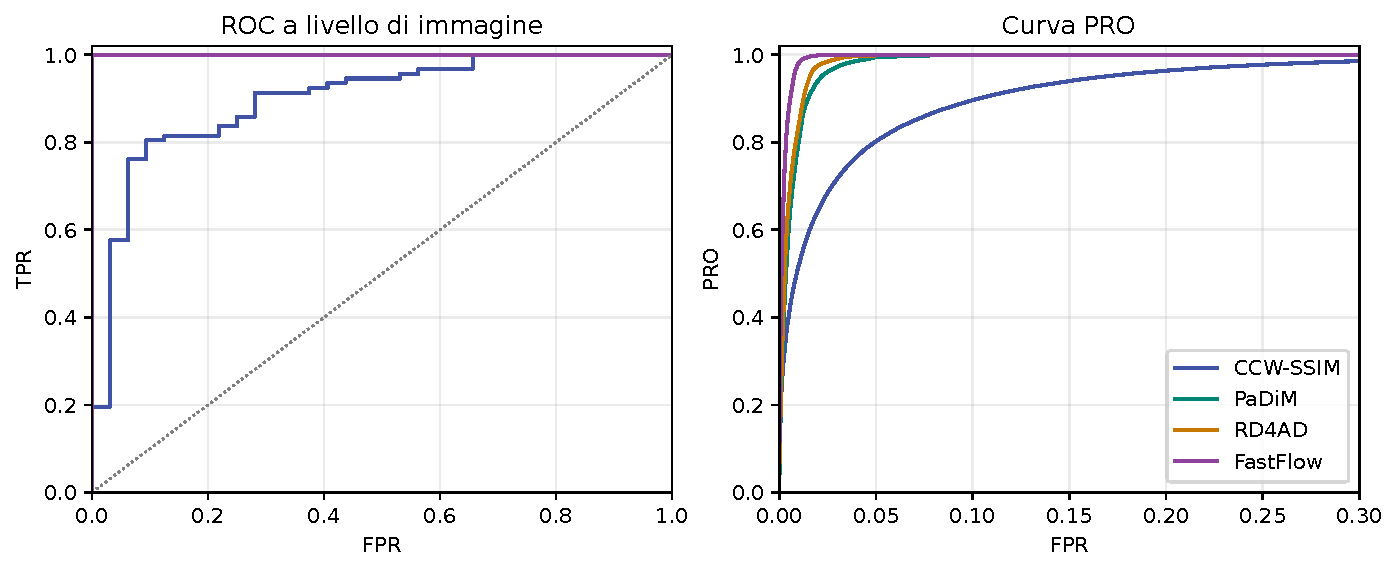
\includegraphics[width=\textwidth]{figure/capitolo_4/curve_roc_pro.pdf}
\caption{Curve ROC a livello di immagine e curve PRO ricavate dai punti archiviati dal valutatore. Le curve ROC di PaDiM, RD4AD e FastFlow si sovrappongono. Le aree riportate nel testo sono quelle salvate nei risultati, non una nuova integrazione dei punti visualizzati.}
\label{fig:cap4-curve}
\end{figure}

\subsection{Risultati a soglia e casi di errore}

Le aree sotto le curve descrivono il comportamento al variare della soglia. Per esaminare le decisioni sulle singole immagini e la segmentazione dei pixel, la Tabella~\ref{tab:cap4-soglie} affianca a queste misure i risultati nei punti operativi selezionati dal valutatore.

\begin{table}[htbp]
\centering
\small
\begin{tabularx}{\textwidth}{Yrrrr}
\hline
Metrica & CCW-SSIM & PaDiM & RD4AD & FastFlow \\
\hline
F1 massimo immagini & 0,9081 & 1,0000 & 1,0000 & 1,0000 \\
F1 massimo pixel & 0,3840 & 0,4243 & 0,4981 & 0,6161 \\
FPR con TPR $\geq 95\%$ & 0,5312 & 0,0000 & 0,0000 & 0,0000 \\
\hline
\end{tabularx}
\caption{Metriche a soglia. Le soglie di massimo F1 sono selezionate sul insieme di test; l'FPR dell'ultima riga riguarda la classificazione delle immagini.}
\label{tab:cap4-soglie}
\end{table}

Alla soglia che massimizza l'F1 a livello di immagine, CCW-SSIM identifica 84 immagini difettose e ne omette 8; classifica correttamente 23 immagini normali e segnala come anomale le altre 9. La precisione è circa 0,9032 e il richiamo circa 0,9130. Per gli altri tre metodi, alla rispettiva soglia ottimale, non si osservano falsi positivi o falsi negativi a livello di immagine.

Il comportamento cambia imponendo un richiamo di almeno il 95\%: per CCW-SSIM l'FPR sale a 0,5312, corrispondente a 17 immagini normali segnalate su 32. Il valore illustra il costo, su questo insieme di dati, della riduzione delle omissioni. Non va confuso con i nove falsi positivi alla soglia di massimo F1, poiché i due criteri selezionano punti operativi differenti.

A livello di pixel, i massimi F1 sono sensibilmente inferiori alle AUROC pixel. Un buon ordinamento dei punteggi non implica infatti che esista una soglia capace di delineare il difetto con precisione elevata: possono rimanere aloni, risposte sullo sfondo o parti della regione non rilevate. La Tabella~\ref{tab:cap4-precisione} esplicita questo compromesso.

\begin{table}[htbp]
\centering
\begin{tabular}{lrrr}
\hline
Modello & Precisione pixel & Richiamo pixel & F1 pixel \\
\hline
CCW-SSIM & 0,3704 & 0,3986 & 0,3840 \\
PaDiM & 0,3159 & 0,6463 & 0,4243 \\
RD4AD & 0,3999 & 0,6603 & 0,4981 \\
FastFlow & 0,5233 & 0,7488 & 0,6161 \\
\hline
\end{tabular}
\caption{Precisione e richiamo alla soglia globale di massimo F1 pixel di ciascun modello, sul campionamento previsto dal valutatore.}
\label{tab:cap4-precisione}
\end{table}

PaDiM recupera una quota di pixel anomali maggiore di CCW-SSIM, ma presenta una precisione inferiore. RD4AD migliora entrambi i valori rispetto a PaDiM, mentre FastFlow ottiene il miglior compromesso osservato. Anche per FastFlow una precisione di 0,5233 indica che, alla soglia considerata, una parte consistente dei pixel segnalati non appartiene alle annotazioni del difetto. L'esito favorevole nel riconoscimento dell'immagine non deve quindi essere trasferito automaticamente alla precisione della segmentazione.

L'interpretazione di questi punti operativi dipende dalla scala del punteggio di ciascun modello. Il valutatore normalizza punteggi originariamente differenti, che non rappresentano probabilità calibrate: le soglie numeriche vanno quindi riferite alla rispettiva pipeline. Il loro uso su dati futuri richiederebbe una selezione su un insieme di validazione indipendente, come discusso nella Sezione~\ref{sec:cap4-limiti}.

\subsection{Costi osservati nella fase di apprendimento}

Accanto alle prestazioni, i tempi registrati descrivono il lavoro necessario ad adattare ciascuna pipeline al materiale. La Tabella~\ref{tab:cap4-costi} li mette in relazione con i passaggi sui dati e gli aggiornamenti dei parametri, distinguendo la stima statistica di PaDiM dall'ottimizzazione iterativa degli altri modelli.

\begin{table}[htbp]
\centering
\small
\begin{tabularx}{\textwidth}{Yrrr}
\hline
Pipeline & Passaggi sui dati & Aggiornamenti & Tempo (min) \\
\hline
CCW-SSIM & 200 & 49\,000 & 374,1 \\
PaDiM & 1 & 0 & 0,2 \\
RD4AD & 200 & 3\,200 & 8,7 \\
FastFlow & 200 & 6\,200 & 11,5 \\
\hline
\end{tabularx}
\caption{Tempi della fase di apprendimento o adattamento registrati nelle esecuzioni su GPU NVIDIA RTX 4070 Ti. Per PaDiM l'adattamento consiste nella stima statistica, senza aggiornamenti tramite discesa del gradiente.}
\label{tab:cap4-costi}
\end{table}

PaDiM richiede il tempo di adattamento più basso, mentre CCW-SSIM presenta quello più alto. RD4AD e FastFlow si collocano tra questi estremi. I tempi non rappresentano un confronto a parità di lavoro: differiscono il numero di aggiornamenti, il batch, la precisione numerica, la gestione delle patch e l'architettura. Inoltre, i metodi basati su feature utilizzano un pre-addestramento esterno, il cui costo non è incluso nelle misure.

Il risultato consente quindi di discutere il costo locale di preparazione delle pipeline, non la loro efficienza complessiva. Non sono disponibili qui misure omogenee di latenza, numero di immagini elaborate per unità di tempo e memoria durante l'inferenza; il tempo di addestramento non può sostituirle né verificare le dichiarazioni di velocità dei lavori originali.

\section{Analisi qualitativa e confronto caso per caso}
\label{sec:cap4-qualitativo}

Le differenze tra AUROC, AU-PRO e F1 rendono utile osservare come i punteggi si distribuiscano nelle immagini. Le figure affiancano l'immagine originale, la maschera annotata e le quattro mappe di anomalia. Il contorno verde sulle mappe indica il riferimento annotato, non una segmentazione prodotta dal modello. Per mantenere una scala coerente tra esempi dello stesso metodo, la visualizzazione applica una normalizzazione min--max basata sull'intero insieme delle mappe di test di ciascuna pipeline:
\begin{equation}
\widetilde{S}_m(x)=\frac{S_m(x)-a_m}{b_m-a_m},
\end{equation}
dove $a_m$ e $b_m$ sono rispettivamente il minimo e il massimo delle mappe del modello $m$. Non viene normalizzata ogni immagine separatamente. Questa trasformazione serve soltanto alla visualizzazione e non modifica le metriche archiviate. Non coincide necessariamente con gli estremi ricavati dal campionamento usato per l'F1 pixel.

Poiché ciascun modello mantiene una propria scala, la stessa tonalità in due pannelli non esprime una probabilità di anomalia equivalente. Il confronto visivo riguarda posizione, forma ed estensione delle risposte. La classificazione dipende invece dal massimo della mappa e dalla soglia globale del modello: una risposta su parte del difetto può essere sufficiente a segnalare l'immagine, mentre una zona luminosa in un campione normale va interpretata rispetto a quella soglia. I conteggi per tipologia riportati nel seguito descrivono le decisioni sulle immagini; la qualità della segmentazione è valutata dalle metriche a livello di pixel e regionali.

Per ciascuna tipologia di difetto è stato scelto il primo file in ordine lessicografico, \texttt{000.png}. La regola rende la selezione riproducibile, ma non garantisce che i campioni siano rappresentativi dell'intera tipologia. Sono aggiunti due esempi diagnostici: l'immagine normale con il massimo punteggio CCW-SSIM e un difetto omesso da tale modello. La Tabella~\ref{tab:cap4-fn} fornisce il contesto quantitativo delle omissioni sull'intero insieme di test, prima della lettura dei singoli esempi.

\begin{table}[htbp]
\centering
\begin{tabular}{lrrrr}
\hline
Difetto & CCW-SSIM & PaDiM & RD4AD & FastFlow \\
\hline
\texttt{color} & 2/19 & 0/19 & 0/19 & 0/19 \\
\texttt{cut} & 1/19 & 0/19 & 0/19 & 0/19 \\
\texttt{fold} & 0/17 & 0/17 & 0/17 & 0/17 \\
\texttt{glue} & 4/19 & 0/19 & 0/19 & 0/19 \\
\texttt{poke} & 1/18 & 0/18 & 0/18 & 0/18 \\
\hline
Totale & 8/92 & 0/92 & 0/92 & 0/92 \\
\hline
\end{tabular}
\caption{Falsi negativi a livello di immagine sul numero di campioni difettosi. Per ogni modello si mantiene la stessa soglia globale di massimo F1 immagini, senza ottimizzarla per tipologia.}
\label{tab:cap4-fn}
\end{table}

\subsection{Alterazione cromatica: \texttt{color}}

Nel campione \texttt{color/000.png} il difetto occupa una piccola zona nella parte inferiore destra dell'immagine. PaDiM, RD4AD e FastFlow producono una risposta riconoscibile nella posizione annotata. PaDiM presenta una distribuzione più regolare e a blocchi, RD4AD una risposta più compatta, mentre FastFlow evidenzia il difetto con un nucleo intenso e una risposta anche nelle aree circostanti. La mappa CCW-SSIM è maggiormente influenzata dalla tessitura diffusa del materiale e mostra un contrasto locale meno evidente.

Il contrasto locale poco evidente di CCW-SSIM si accompagna al riconoscimento di 17 delle 19 immagini \texttt{color} alla soglia globale di massimo F1. L'esempio invita quindi a esaminare la relazione tra risposta cromatica e tessitura del materiale. Il contributo specifico del colore alla funzione di perdita sarà discusso nel confronto con la fonte, poiché la sua misura richiede un'ablazione controllata rispetto alla variante priva di tale componente.

\begin{figure}[htbp]
\centering
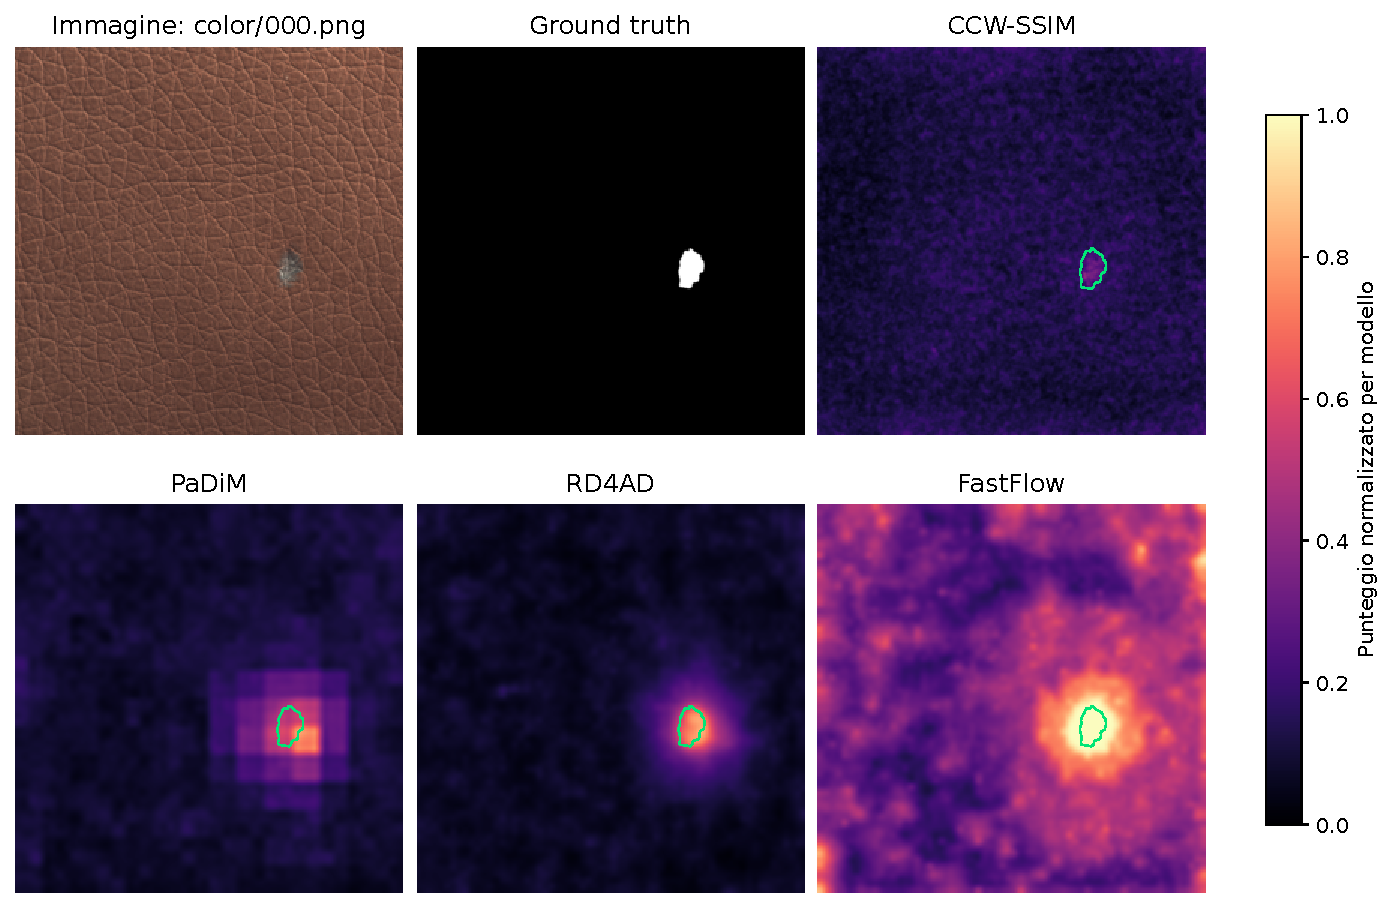
\includegraphics[width=\textwidth]{figure/capitolo_4/leather_color_000.pdf}
\caption{Confronto qualitativo sul campione \texttt{color/000.png}. Il contorno verde rappresenta la regione annotata.}
\label{fig:cap4-color}
\end{figure}

\subsection{Taglio: \texttt{cut}}

Il campione \texttt{cut/000.png} contiene un difetto sottile, prevalentemente orizzontale. I tre metodi basati su feature rispondono nell'area corretta, ma la regione ad alto punteggio si estende oltre la geometria del taglio. Questo esempio rende visibile la distinzione tra individuare la posizione del difetto e ricostruirne precisamente il contorno. La risposta PaDiM è più squadrata; quelle di RD4AD e FastFlow sono più continue, pur mantenendo un'estensione superiore alla maschera.

CCW-SSIM presenta una mappa granulare nella quale il difetto emerge meno nettamente rispetto allo sfondo; sull'intera tipologia viene omessa una sola immagine su 19. Il caso richiama soprattutto l'attenzione sui bordi: per una struttura sottile, ricampionamento e filtraggio possono influenzare l'estensione visibile della risposta. Gli esperimenti disponibili descrivono l'esito della pipeline completa e non isolano il contributo di questi passaggi.

\begin{figure}[htbp]
\centering
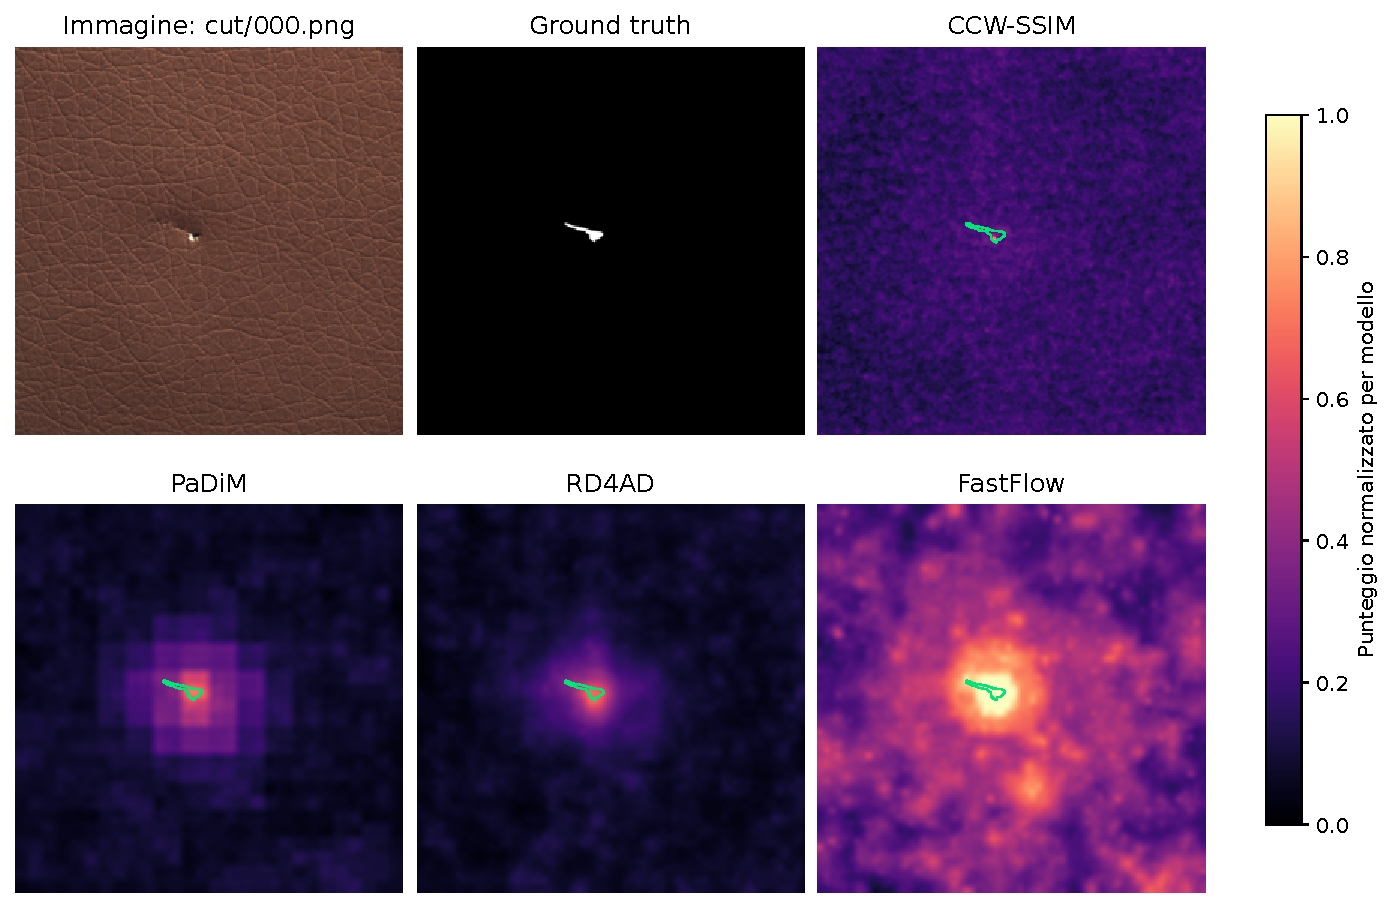
\includegraphics[width=\textwidth]{figure/capitolo_4/leather_cut_000.pdf}
\caption{Confronto sul campione \texttt{cut/000.png}: la risposta nell'area corretta non implica una segmentazione aderente al taglio.}
\label{fig:cap4-cut}
\end{figure}

\subsection{Piega: \texttt{fold}}

In \texttt{fold/000.png} la regione difettosa è allungata e si trova nella parte superiore sinistra. PaDiM, RD4AD e FastFlow individuano tale zona, con risposte che ne comprendono anche il contesto. CCW-SSIM conserva una risposta diffusa alla texture e un'evidenza locale meno netta alla scala di visualizzazione adottata.

CCW-SSIM riconosce tutte le 17 immagini \texttt{fold} alla soglia di massimo F1 immagini. La risposta diffusa osservata nel pannello convive quindi con un riconoscimento completo della tipologia nel test. Il caso mostra come il massimo della mappa possa sostenere la decisione sull'immagine anche quando la regione difettosa emerge con un contrasto visivo limitato.

\begin{figure}[htbp]
\centering
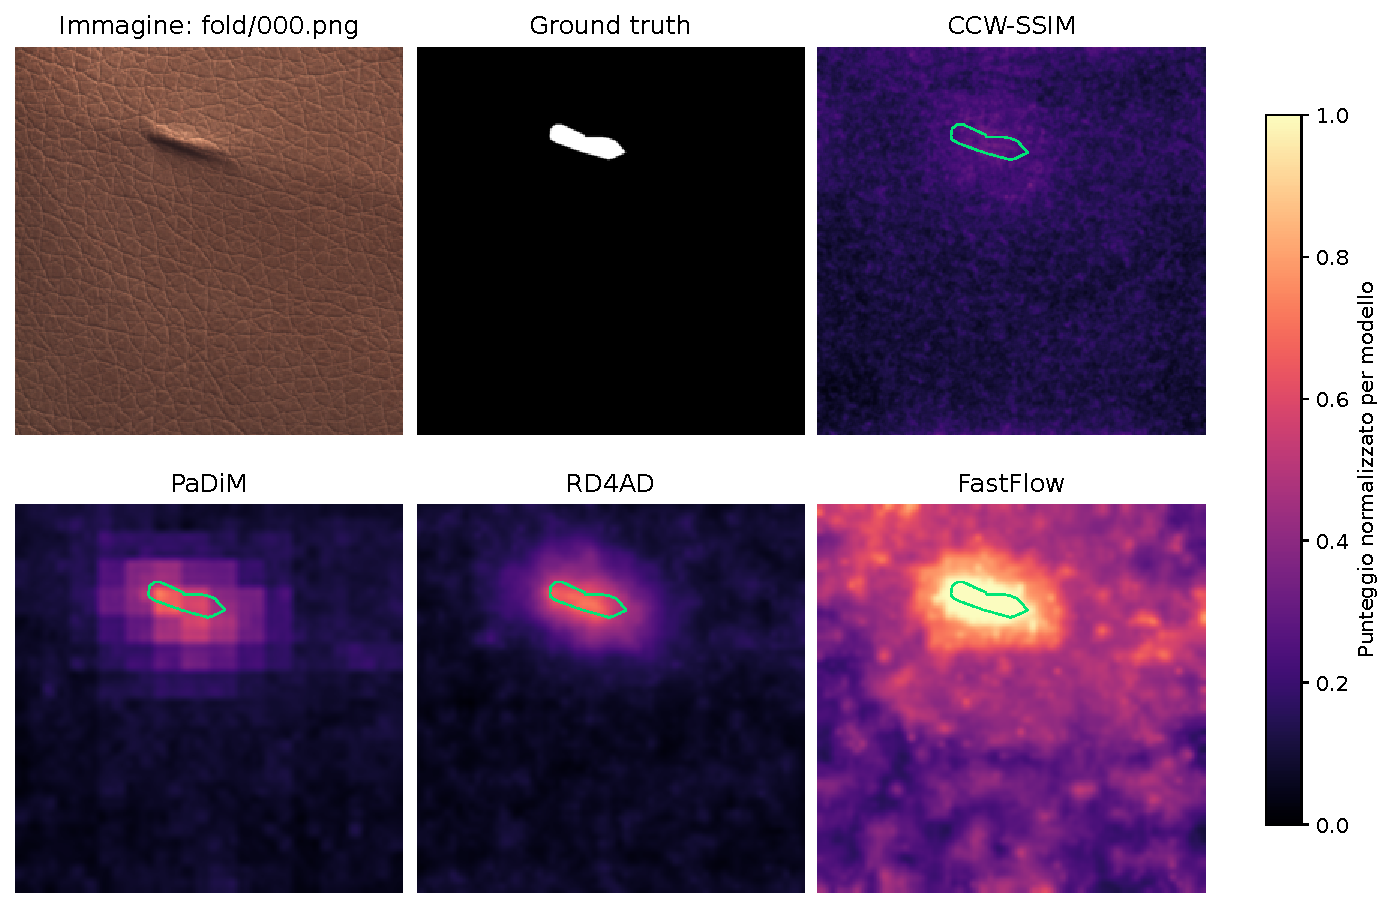
\includegraphics[width=\textwidth]{figure/capitolo_4/leather_fold_000.pdf}
\caption{Confronto sul campione \texttt{fold/000.png}, caratterizzato da un difetto allungato.}
\label{fig:cap4-fold}
\end{figure}

\subsection{Residuo di colla: \texttt{glue}}

Nel campione \texttt{glue/000.png} la regione annotata è compatta e presenta variazioni di aspetto al suo interno. Le mappe PaDiM e RD4AD rispondono in modo non uniforme nella zona difettosa; FastFlow produce un nucleo più estesamente intenso. CCW-SSIM mostra risposte soprattutto su piccole porzioni e variazioni locali, senza riprodurre con altrettanta evidenza l'intera area annotata.

Quattro degli otto falsi negativi di CCW-SSIM appartengono a \texttt{glue}: sono quattro omissioni su 19 campioni, il numero più alto tra le tipologie considerate. La Figura~\ref{fig:cap4-glue-fn} aggiunge \texttt{glue/001.png}, il primo falso negativo in ordine lessicografico di questa tipologia. Il campione è selezionato per documentare un errore effettivo, non per rappresentare un caso medio. La sua omissione è determinata dal punteggio globale dell'immagine alla soglia considerata, non dall'assenza di qualunque risposta visibile sulla mappa.

\begin{figure}[htbp]
\centering
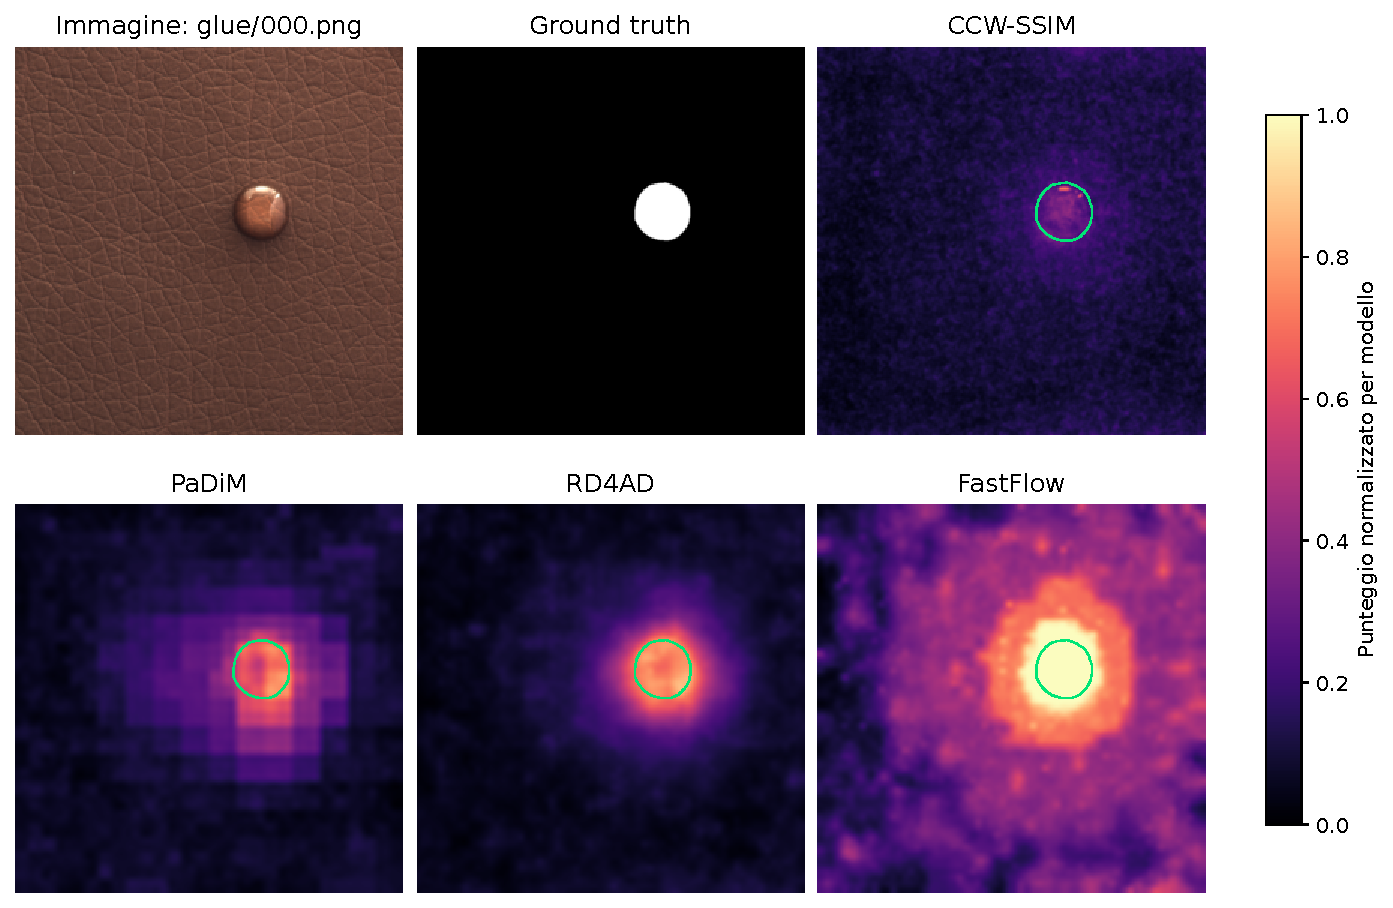
\includegraphics[width=\textwidth]{figure/capitolo_4/leather_glue_000.pdf}
\caption{Confronto sul campione \texttt{glue/000.png}.}
\label{fig:cap4-glue}
\end{figure}

\begin{figure}[htbp]
\centering
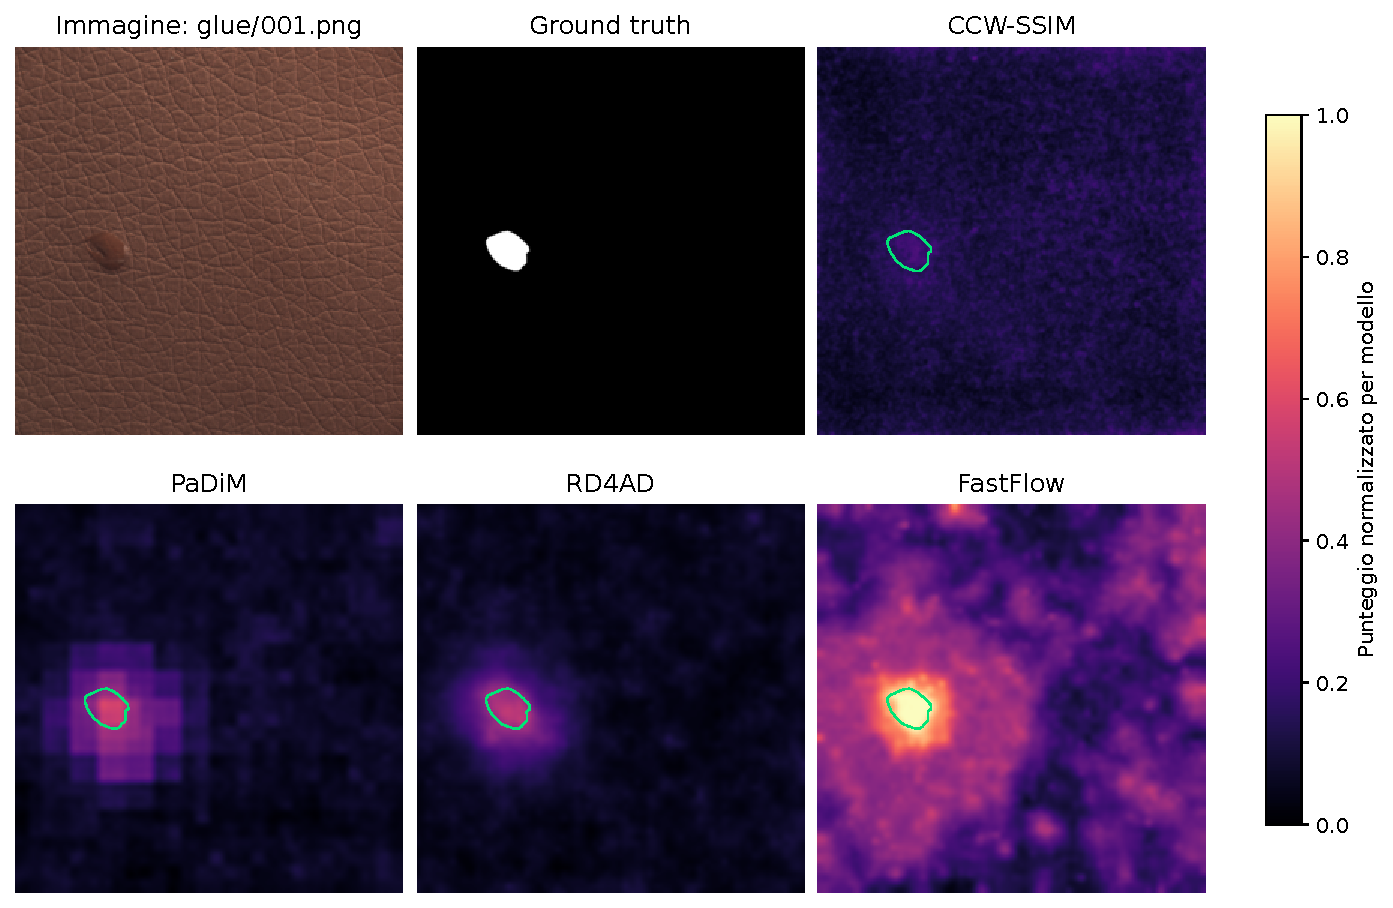
\includegraphics[width=\textwidth]{figure/capitolo_4/leather_glue_001.pdf}
\caption{Campione \texttt{glue/001.png}, falso negativo di CCW-SSIM alla soglia globale di massimo F1 immagini. Gli altri tre modelli lo classificano correttamente alle rispettive soglie.}
\label{fig:cap4-glue-fn}
\end{figure}

\subsection{Perforazione: \texttt{poke}}

In \texttt{poke/000.png} il difetto è piccolo e si trova nella parte inferiore sinistra. I tre modelli basati su feature presentano una risposta localizzata, più ampia del riferimento annotato. CCW-SSIM mostra una risposta meno distinguibile dalla texture circostante. Per un difetto di dimensioni ridotte, un'estensione della mappa oltre il contorno può incidere sulla precisione anche quando il centro della risposta è corretto.

CCW-SSIM omette una delle 18 immagini \texttt{poke} alla soglia globale scelta, mentre gli altri metodi le riconoscono tutte. Rispetto agli esempi precedenti, la piccola area annotata mette in evidenza il peso delle risposte circostanti: una localizzazione centrata sul difetto può comunque includere una quota rilevante di pixel normali.

\begin{figure}[htbp]
\centering
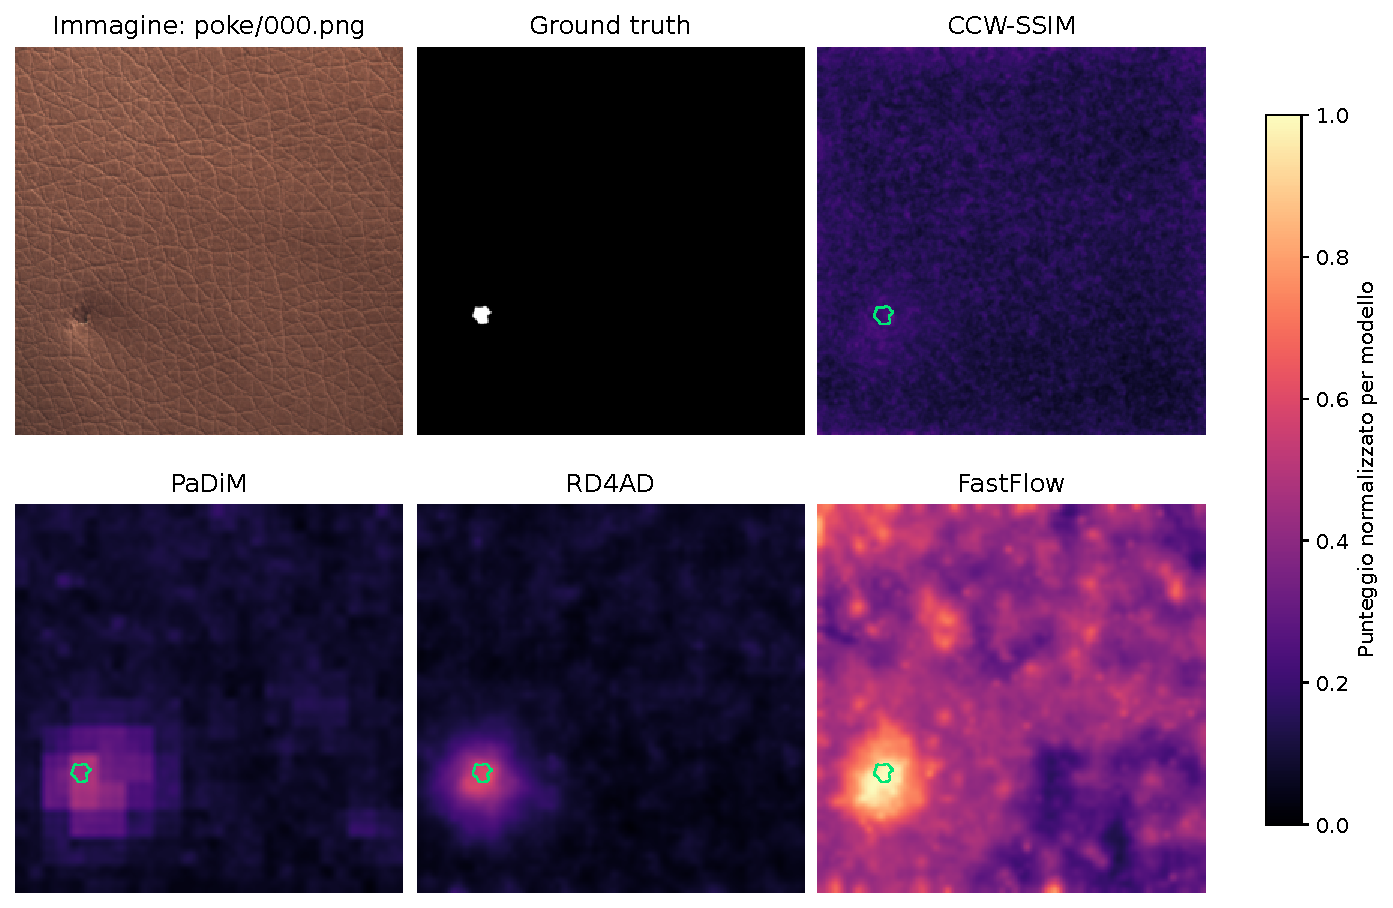
\includegraphics[width=\textwidth]{figure/capitolo_4/leather_poke_000.pdf}
\caption{Confronto sul campione \texttt{poke/000.png}, con difetto di piccole dimensioni.}
\label{fig:cap4-poke}
\end{figure}

\subsection{Immagine normale e falso positivo}

Il campione \texttt{good/030.png} è l'immagine normale con il massimo punteggio CCW-SSIM. La maschera di riferimento è vuota. La mappa CCW-SSIM contiene risposte diffuse alla tessitura e picchi locali: il massimo supera la soglia di classificazione e rende questa immagine uno dei nove falsi positivi del modello.

Anche le altre pipeline producono mappe non uniformi su questa immagine normale, ma i rispettivi punteggi rimangono al di sotto delle soglie globali di massimo F1 immagini. Per CCW-SSIM, invece, il picco determina una segnalazione errata. Il caso collega così la risposta alla tessitura alla scelta di aggregare la mappa mediante massimo e motiva un possibile approfondimento su aggregazioni alternative, il cui beneficio rimane da verificare.

\begin{figure}[htbp]
\centering
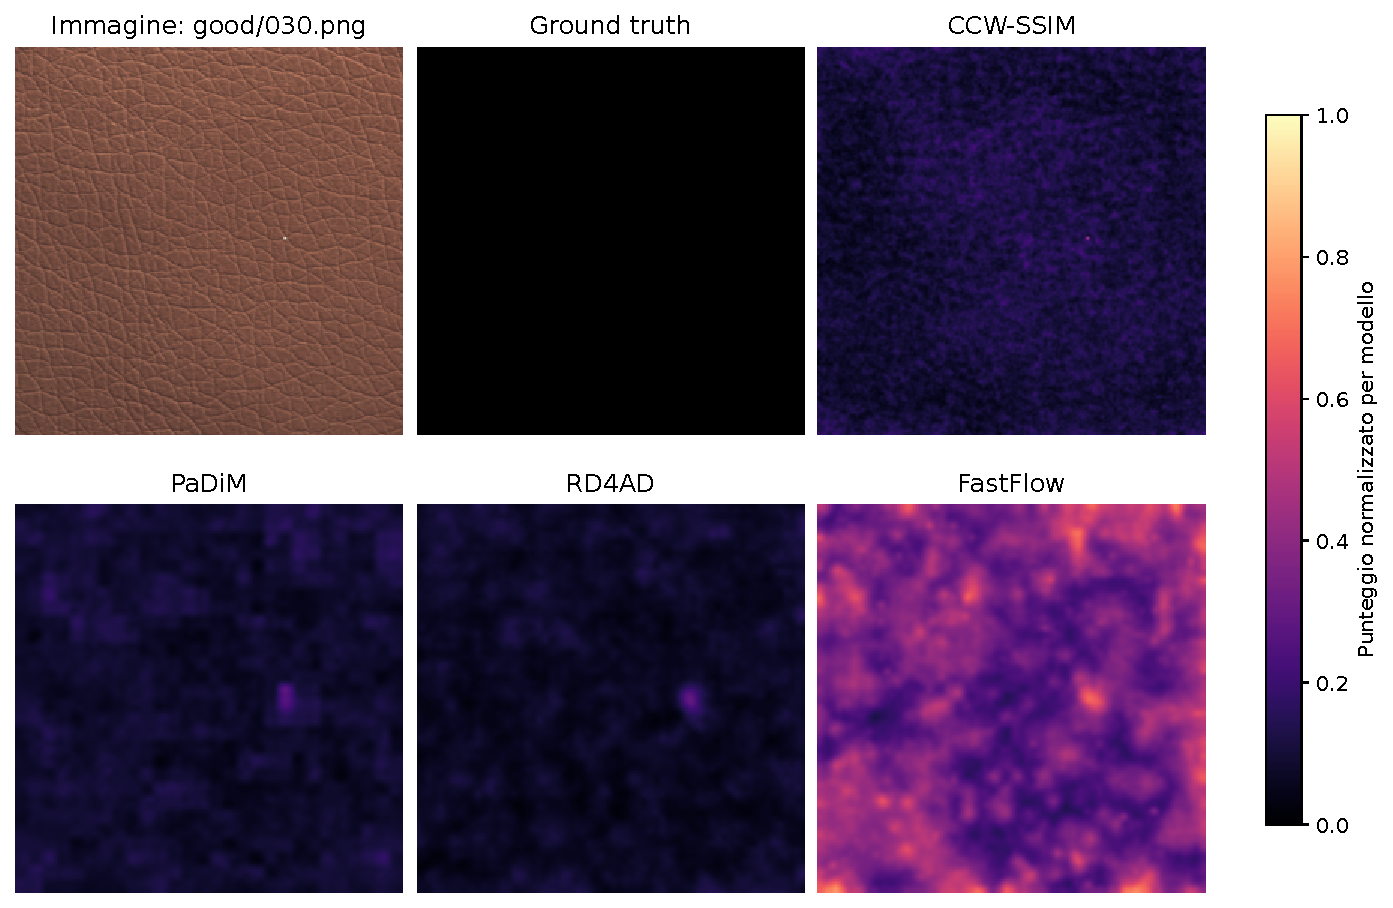
\includegraphics[width=\textwidth]{figure/capitolo_4/leather_good_030.pdf}
\caption{Immagine normale \texttt{good/030.png}, falso positivo di CCW-SSIM alla soglia di massimo F1 immagini. L'assenza di regioni annotate è mostrata dalla maschera vuota.}
\label{fig:cap4-good}
\end{figure}

\subsection{Sintesi della lettura qualitativa}

Negli esempi selezionati, PaDiM mostra risposte più regolari e a blocchi, RD4AD risposte più compatte e FastFlow nuclei intensi accompagnati, in alcuni casi, da un'attivazione più diffusa del contesto. CCW-SSIM presenta mappe più granulari, nelle quali la texture normale rimane visibile e il contrasto del difetto può essere ridotto. Queste descrizioni riguardano i pannelli esaminati e non sostituiscono un'analisi quantitativa di tutte le mappe.

La lettura delle figure è coerente con due risultati complessivi: i metodi basati su feature individuano la zona difettosa nei campioni mostrati, ma mantengono imprecisioni di estensione; CCW-SSIM può segnalare un difetto senza coprirlo interamente e può attribuire un punteggio elevato anche a un'immagine normale. Non è invece giustificato attribuire le differenze alla sola risoluzione, al solo pre-addestramento o alla sola funzione di perdita: tali fattori non sono stati variati separatamente.

\FloatBarrier

\section{Confronto con le pubblicazioni di riferimento}
\label{sec:cap4-letteratura}

Le metriche e gli esempi visivi delineano il comportamento delle pipeline nel caso di studio. Per metterlo in relazione con le proposte originali, occorre confrontare sia i valori pubblicati sia le condizioni in cui sono stati ottenuti. Si considerano quindi i risultati di \texttt{leather}, quando disponibili, mantenendoli distinti dalle medie sulle quindici categorie di MVTec AD.

La Tabella~\ref{tab:cap4-paper} affianca i risultati locali ai valori pubblicati per le metriche con una corrispondenza nominale. Gli scarti sono espressi in punti percentuali e sono soltanto descrittivi: la tabella non presuppone identità dei protocolli. CCW-SSIM viene discusso separatamente, poiché la diversa definizione dell'area impedisce di riportare uno scarto equivalente.

\begin{table}[htbp]
\centering
\small
\begin{tabularx}{\textwidth}{lYrrr}
\hline
Metodo & Metrica & Fonte (\%) & Locale (\%) & Scarto (p.p.) \\
\hline
PaDiM & AUROC pixel & 99,20 & 99,11 & $-0,09$ \\
 & PRO & 97,80 & 97,86 & $+0,06$ \\
RD4AD & AUROC immagini & 100,00 & 100,00 & $0,00$ \\
 & AUROC pixel & 99,40 & 99,42 & $+0,02$ \\
 & PRO & 99,10 & 98,33 & $-0,77$ \\
FastFlow & AUROC immagini & 100,00 & 100,00 & $0,00$ \\
 & AUROC pixel & 99,50 & 99,68 & $+0,18$ \\
\hline
\end{tabularx}
\caption{Riscontro descrittivo su \texttt{leather} con le tabelle originali di PaDiM, Reverse Distillation e FastFlow. La misura regionale locale è l'AU-PRO definita nel protocollo dell'elaborato; la corrispondenza esatta dei valutatori non è accertata per tutte le fonti. Lo scarto è locale meno fonte e non indica significatività statistica.}
\label{tab:cap4-paper}
\end{table}

\subsection{PaDiM}

Nella Tabella III del lavoro di Defard et al.~\cite{Defard_et_al._2021}, la configurazione PaDiM con Wide ResNet-50-2 e 550 dimensioni riporta per \texttt{leather} un'AUROC pixel del 99,2\% e un PRO-score del 97,8\%. I valori locali, rispettivamente 99,11\% e 97,86\%, sono prossimi a quelli pubblicati. Questo riscontro sostiene la coerenza del comportamento di localizzazione osservato.

Per interpretare questo allineamento occorre considerare il preprocessing. Il lavoro originale prevede ridimensionamento a 256 pixel e ritaglio centrale a 224, mentre la configurazione locale ridimensiona direttamente a 224. Possono inoltre differire dettagli del valutatore e della selezione delle feature.

La differenza di preprocessing è concreta: il ritaglio conserva la scala della parte centrale dell'immagine ridimensionata e ne esclude i margini, mentre il ridimensionamento diretto mantiene l'intero campo visivo a una scala diversa. Questo modifica la corrispondenza tra texture, difetti e posizioni delle feature statistiche. È un fattore plausibile per leggere i piccoli scarti, ma il suo effetto non è stato misurato separatamente. Anche il rapido adattamento locale è coerente con l'assenza di addestramento della rete descritta dalla pubblicazione; non costituisce invece una verifica dei suoi tempi assoluti, ottenuti con hardware e implementazione differenti.

\subsection{Reverse Distillation}

Le Tabelle 1 e 2 di Deng e Li~\cite{Deng_et_al._2022} riportano per \texttt{leather}, alla risoluzione di 256 pixel, un'AUROC immagini del 100\%, un'AUROC pixel del 99,4\% e un PRO del 99,1\%. Nell'esecuzione locale RD4AD raggiunge rispettivamente il 100\%, il 99,42\% e il 98,33\%.

La discriminazione delle immagini e l'AUROC pixel risultano quindi prossime ai valori pubblicati, mentre tra i due valori regionali vi è uno scarto descrittivo di circa 0,77 punti percentuali. La verifica del codice ufficiale \cite{Deng_RD4AD_code_2022} accerta però protocolli differenti: il riferimento calcola il PRO per ciascuna immagine difettosa, con 200 soglie, poi media le aree; il valutatore locale costruisce un'unica curva globale sulle 124 immagini, includendo quelle normali. Le due procedure pesano diversamente regioni e falsi positivi. Lo scarto non misura quindi una perdita del modello a parità di valutazione.

I principali parametri di addestramento coincidono con quelli dichiarati nella fonte: 200 epoche, batch da 16 immagini e Adam con tasso di apprendimento pari a 0,005 e coefficienti $(0{,}5,0{,}999)$. Il codice ufficiale valuta e filtra a $256\times256$, mentre qui le mappe sono interpolate a $1024\times1024$ prima del filtro con $\sigma=4$: lo stesso valore numerico non corrisponde alla stessa scala spaziale. È verificata la differenza di procedura, non il suo contributo quantitativo al risultato. Per isolare le cause servirebbe applicare entrambi i protocolli a predizioni omogenee, senza modificare retrospettivamente il confronto locale.

\subsection{FastFlow}

La Tabella 2 di Yu et al.~\cite{Yu_et_al._2021} riporta per \texttt{leather} un'AUROC immagini del 100\% e un'AUROC pixel del 99,5\%. L'esecuzione locale ottiene il 100\% e il 99,68\%. I risultati confermano, nel perimetro considerato, la buona separazione delle immagini e l'elevata capacità di localizzazione descritta nella pubblicazione.

Il porting adottato utilizza la configurazione Wide ResNet-50-2 documentata nel Capitolo~\ref{chap:implementazione}, mentre la pubblicazione considera diverse architetture di estrazione delle feature. L'identità completa con la configurazione sottostante al valore pubblicato non è stabilita. Il lieve scarto positivo va quindi interpretato insieme alle scelte di implementazione e di apprendimento.

La fonte descrive 500 epoche e batch da 32, mentre il progetto usa 200 epoche e batch da 8, mantenendo tasso di apprendimento $10^{-3}$ e decadimento dei pesi $10^{-5}$. Cambiano così il regime di ottimizzazione e il numero di aggiornamenti. Il vantaggio descrittivo di 0,18 punti percentuali non può essere attribuito a una modifica specifica senza prove controllate. Il confronto sostiene la capacità di produrre punteggi discriminanti nel caso di studio; le proprietà di efficienza in inferenza discusse dalla pubblicazione richiederebbero invece misure di latenza e numero di immagini elaborate per unità di tempo, distinte dai tempi di addestramento qui riportati.

\subsection{CCW-SSIM e il ruolo dell'informazione cromatica}

La fonte di Berasi~\cite{Berasi_2023} ha come obiettivo centrale l'integrazione dell'informazione cromatica nella misura strutturale utilizzata da un autoencoder. Il confronto tra varianti della funzione di perdita è quindi essenziale per valutarne il contributo. Il presente lavoro include CCW-SSIM nel confronto con tre pipeline basate su feature, ma non contiene l'ablazione controllata rispetto alla variante CW-SSIM. Non può pertanto confermare né confutare direttamente il vantaggio della componente cromatica.

Un'ulteriore distinzione riguarda le metriche. La Tabella 1 della fonte riporta per \texttt{leather} il valore 0,982 relativo alla curva ROC; nella sezione sulle prestazioni, la fonte specifica una normalizzazione dell'area limitata a FPR pari a 0,3. La nostra AUROC pixel, pari a 0,9707, integra invece la curva completa. Anche l'AU-PRO locale non è la stessa misura, perché integra la copertura delle regioni anziché il tasso di veri positivi pixel. Nessuno dei due valori consente quindi un confronto diretto con 0,982.

Il risultato locale di CCW-SSIM va dunque letto rispetto alla pipeline utilizzata. La fonte distingue il beneficio cromatico all'interno dell'approccio ricostruttivo dal confronto con metodi più sofisticati dello stato dell'arte. Per approfondire tale beneficio nel progetto occorre mantenere fissi architettura, dati e valutatore e variare la componente della perdita.

La verifica del percorso effettivo individua inoltre differenze nella componente cromatica, esplicitate nel Capitolo~\ref{chap:implementazione}: errore quadratico anziché distanza euclidea, aggregazione globale durante l'addestramento e coefficienti differenti in inferenza. Queste scelte preservano l'idea di combinare struttura e colore, ma non permettono di trasferire automaticamente alla variante locale il beneficio cromatico dimostrato dalla fonte.

Per approfondire le scelte di implementazione, un test diagnostico del checkpoint esistente, senza addestramento e senza sostituire le mappe ufficiali, ha elaborato dodici patch $128\times128$ estratte da quattro posizioni fissate nelle prime tre immagini normali di test. In tali patch la luminanza ricostruita è già positiva. L'RMSE sul canale $L^*$ è compreso tra 2,08 e 7,03 unità Lab prima dell'inversione e tra 63,90 e 72,02 dopo. L'inversione non è dunque giustificata come correzione necessaria in questi campioni. Non cambia però la perdita CW-SSIM misurata, che rimane pari a 0,153519: il modulo del prodotto dei coefficienti rende la misura insensibile all'inversione globale del segno. La componente cromatica usa soltanto $a^*$ e $b^*$. L'inversione del canale $L^*$ non spiega pertanto il divario nelle metriche della mappa.

Nel medesimo test, la perdita totale è 0,153527, superiore alla componente strutturale di circa $8{,}43\times10^{-6}$. La correzione cromatica media prima della moltiplicazione è circa $9{,}96\times10^{-6}$ durante l'addestramento; il coefficiente di inferenza darebbe circa 0,00448 prima della media spaziale. Questi valori accertano una piccola incidenza cromatica sul valore della perdita in queste patch e una diversa pesatura in inferenza, non dimostrano l'effetto sui gradienti o sulle prestazioni. Il test non sostituisce un'ablazione.

Una verifica complementare riguarda la posizione dei picchi che determinano gli errori di classificazione. L’analisi spaziale delle mappe archiviate localizza il massimo di otto dei nove falsi positivi entro tre pixel dal bordo. Il campione \texttt{good/030.png}, già discusso, ha invece il massimo all'interno dell'immagine. Ciò individua una criticità del punteggio aggregato mediante massimo e della risposta periferica, senza provare quale componente la generi. Non viene applicata una correzione dei bordi scelta sulle etichette del test; i risultati principali conservano la mappa originale del protocollo originale.

La previsione su patch da $256\times256$ con stride 16 è allineata alla procedura descritta dalla fonte. Il riferimento a 50\,000 patch normali di addestramento non va invece equiparato ai 49\,000 aggiornamenti locali: un aggiornamento utilizza un batch di patch e le due quantità misurano aspetti diversi dell'esperimento. Le mappe e gli errori analizzati offrono una spiegazione descrittiva del risultato locale, mostrando risposte alla texture normale e copertura parziale di alcuni difetti. Non permettono di stabilire perché la prestazione differisca da quella della pubblicazione, prima ancora di rendere omogenee le metriche.

\subsection{Interpretazione degli scostamenti}

Il confronto distingue tre livelli di evidenza. Il primo è il risultato misurato: per PaDiM gli scarti sono piccoli, per RD4AD emerge soprattutto una differenza nel PRO e per FastFlow le AUROC sono in linea o lievemente superiori ai valori riportati. Il secondo comprende le differenze documentate, come il preprocessing di PaDiM, il regime di addestramento di FastFlow e la metrica della fonte CCW-SSIM. Il terzo comprende le ipotesi esplicative, tra cui la sensibilità del PRO ai bordi e la variabilità delle esecuzioni. Soltanto i primi due livelli sono verificati dal materiale disponibile; il terzo richiede prove dedicate.

La consistenza del confronto interno è sostenuta anche dal ricalcolo completo delle mappe archiviate: per ciascuna pipeline sono confermate le tre aree principali e tredici valori aggiuntivi relativi a F1, soglie, precisione, richiamo e scala dei punteggi, senza differenze numeriche rispetto ai file di risultato. Questa verifica collega le metriche ai dati e al valutatore comuni. Il rapporto con le fonti rimane invece condizionato dalle differenze documentate: il protocollo regionale di RD4AD, le condizioni di apprendimento e le misure di efficienza di FastFlow e la variante cromatica locale di CCW-SSIM.

\section{Limiti e portata dei risultati}
\label{sec:cap4-limiti}

Il perimetro sperimentale consente di approfondire un materiale attraverso cinque tipologie di difetto. Le conclusioni riguardano quindi \texttt{leather}; una valutazione su altre categorie sarebbe necessaria per esaminare la generalizzazione a materiali e oggetti differenti.

La stabilità delle differenze osservate richiede inoltre repliche. Una sola esecuzione per pipeline non quantifica la variabilità rispetto al seme pseudo-casuale o all'addestramento e non permette di stabilire una superiorità statisticamente significativa. Anche i pixel di una stessa immagine sono correlati: la loro numerosità non equivale a un insieme altrettanto ampio di osservazioni indipendenti.

Il passaggio a un impiego operativo dipende dalla scelta delle soglie e dalla composizione dei dati. Le soglie ottimali sono selezionate sul test stesso e le immagini difettose sono 92 su 124, una proporzione che non descrive necessariamente una linea produttiva. Precisione e F1 possono cambiare al variare della prevalenza delle anomalie. Una valutazione operativa richiederebbe soglie definite su dati separati e misure coerenti con il costo delle omissioni e dei falsi allarmi.

Infine, l'analisi qualitativa si basa su pochi campioni scelti con criteri espliciti. I conteggi per tipologia riguardano la classificazione delle immagini; non sono disponibili in questa analisi metriche di localizzazione separate per ciascun tipo di difetto. Le differenze di pre-addestramento, risoluzione e post-elaborazione impediscono inoltre una spiegazione causale delle differenze osservate. Questi limiti non annullano il confronto, ma ne delimitano le conclusioni.

\section{Discussione complessiva}

Nel caso di studio esaminato, PaDiM, RD4AD e FastFlow separano completamente le immagini normali da quelle difettose. La localizzazione mostra invece differenze: FastFlow ottiene i valori più alti delle metriche considerate, RD4AD segue con prestazioni prossime e PaDiM mantiene risultati elevati con il costo di adattamento più contenuto. Le mappe rendono visibile che il riconoscimento corretto dell'immagine può convivere con risposte più estese del difetto.

CCW-SSIM presenta un costo di apprendimento maggiore, una separazione delle immagini meno efficace e una copertura regionale inferiore. Individua comunque 84 delle 92 immagini difettose alla soglia di massimo F1. Le omissioni e il campione normale analizzato indicano che la relazione tra risposta alla texture, aggregazione del punteggio e localizzazione merita attenzione, senza che gli esperimenti disponibili consentano di isolare il contributo di ciascun fattore.

Il confronto con le fonti colloca questi risultati nel contesto delle configurazioni e delle metriche adottate. Le differenze documentate aiutano a delimitare il riscontro numerico, mentre le spiegazioni causali richiedono esperimenti dedicati. Su questa base, il Capitolo~\ref{chap:conclusioni} ricompone le risposte agli obiettivi iniziali e propone gli approfondimenti necessari per sviluppare il lavoro.
\chapter{Conclusioni e sviluppi futuri}
\label{chap:conclusioni}

\section{Bilancio del lavoro}

Il lavoro ha esaminato come quattro approcci al rilevamento delle anomalie visive industriali descrivano la normalità e riconoscano i difetti. Il confronto tra CCW-SSIM, PaDiM, RD4AD e FastFlow ha collegato i principi dello stato dell'arte alle configurazioni adottate, utilizzando le immagini della categoria \texttt{leather} di MVTec AD e un protocollo comune di valutazione. Le metriche, le mappe di anomalia e i casi di errore hanno permesso di considerare insieme il riconoscimento delle immagini difettose e la localizzazione delle regioni anomale.

PaDiM, RD4AD e FastFlow hanno separato completamente le immagini normali e difettose del test esaminato. La localizzazione ha invece mostrato differenze tra i tre modelli: FastFlow ha ottenuto i valori più elevati delle metriche considerate, seguito da RD4AD e PaDiM. Le mappe hanno reso visibile che una risposta nella posizione corretta può estendersi oltre il contorno annotato; precisione e richiamo hanno descritto il compromesso tra copertura del difetto e segnalazione di pixel normali. Il risultato a livello di immagine va quindi letto insieme alla qualità della localizzazione.

CCW-SSIM ha presentato una separazione delle immagini meno efficace e una copertura regionale inferiore. Negli esempi analizzati, le risposte alla texture normale rendono meno netto il contrasto del difetto e possono contribuire a una segnalazione anche in assenza di anomalie. La lettura dei casi visivi ha così aiutato a comprendere aspetti del comportamento della pipeline che la sola AUROC non descrive pienamente.

Anche i tempi di apprendimento riflettono le differenze tra gli approcci. PaDiM ha richiesto il minor tempo di adattamento locale, poiché stima le statistiche delle feature senza aggiornare l'estrattore. CCW-SSIM ha richiesto il tempo maggiore, mentre RD4AD e FastFlow si sono collocati in posizione intermedia. Le misure descrivono la preparazione delle pipeline nelle condizioni adottate; il costo del pre-addestramento esterno e le risorse necessarie durante l'inferenza richiedono valutazioni distinte.

Il confronto con le pubblicazioni ha mostrato AUROC di PaDiM, RD4AD e FastFlow prossime ai valori riportati per \texttt{leather}. Le differenze di configurazione e valutazione aiutano però a definire la portata di questo riscontro. Per RD4AD cambia il protocollo di calcolo del PRO; per CCW-SSIM differiscono la metrica della fonte e la formulazione della componente cromatica. Le verifiche diagnostiche hanno approfondito alcuni aspetti della variante locale, senza isolare il beneficio del colore rispetto a CW-SSIM. La valutazione di tale contributo rimane quindi una domanda aperta.

Il contributo dell'elaborato consiste in un confronto documentato che mette in relazione prestazioni, costi di adattamento e comportamento delle mappe. La registrazione di dati, configurazioni e risultati permette di ricondurre le osservazioni alle esecuzioni analizzate. Nel caso di studio, questa impostazione ha consentito di riconoscere sia le capacità delle diverse pipeline sia i punti che richiedono un approfondimento sperimentale.

\section{Portata delle conclusioni}

I risultati riguardano un unico materiale e le configurazioni utilizzate nel progetto. Le cinque tipologie di difetto permettono di esaminare manifestazioni diverse delle anomalie all'interno di \texttt{leather}, mentre la generalizzazione ad altri materiali richiede ulteriori esperimenti. Le differenze di risoluzione, pre-addestramento e trattamento delle mappe sono parte del confronto e non sono state isolate mediante prove controllate.

Una sola esecuzione per modello non permette inoltre di quantificare la variabilità dei risultati. I piccoli scarti tra pipeline descrivono le esecuzioni osservate, ma non dimostrano una superiorità statisticamente significativa. Anche la scelta delle soglie delimita il significato delle prestazioni: il massimo F1 è calcolato sul test stesso e la proporzione di immagini difettose può differire da quella di una linea produttiva. Il passaggio all'impiego industriale richiederebbe soglie selezionate su dati separati e una valutazione del compromesso tra omissioni e falsi allarmi in funzione dell'applicazione.

Queste condizioni definiscono anche le priorità per lo sviluppo del lavoro: approfondire i componenti delle pipeline, verificare la stabilità delle prestazioni e valutare il comportamento in condizioni operative differenti.

\section{Sviluppi futuri}

Un primo approfondimento riguarda il contributo dell'informazione cromatica in CCW-SSIM. La diversa pesatura tra addestramento e inferenza motiva una revisione controllata della componente cromatica, con parametri coerenti con la normalizzazione. Il confronto con CW-SSIM, mantenendo invariati architettura, dati, addestramento e valutatore, permetterebbe poi di misurare il beneficio del colore. L'analisi della tipologia \texttt{color} andrebbe affiancata a quella degli altri difetti e delle risposte sulla texture normale. La modifica della perdita richiederebbe un nuovo addestramento e risultati identificati come un esperimento successivo.

La stabilità del confronto potrebbe essere esaminata attraverso repliche con diversi semi pseudo-casuali. All'interno di \texttt{leather}, il calcolo delle metriche di localizzazione per tipologia di difetto completerebbe inoltre i conteggi di classificazione già disponibili. Il confronto con i valutatori originali, soprattutto per il PRO di RD4AD, aiuterebbe a distinguere le differenze di calcolo da quelle delle pipeline.

Un altro sviluppo riguarda la scelta del punto operativo. Un insieme di validazione separato consentirebbe di definire le soglie prima della valutazione sul test. Per CCW-SSIM, il confronto tra il massimo della mappa e aggregazioni alternative permetterebbe di verificare se una minore sensibilità ai picchi isolati riduca i falsi positivi mantenendo il rilevamento dei piccoli difetti.

La valutazione applicativa richiederebbe infine misure di latenza, numero di immagini elaborate per unità di tempo e memoria di inferenza sullo stesso hardware, distinguendo preprocessing, esecuzione del modello e post-elaborazione. Prove controllate con variazioni di illuminazione e colore permetterebbero di esaminare la robustezza alle condizioni di acquisizione; l'estensione ad altri materiali consentirebbe di studiare la generalizzazione.

Il caso di studio mostra quindi l'utilità di affiancare alla capacità di riconoscere un'immagine difettosa l'analisi della localizzazione, delle soglie e dei costi osservati. I metodi basati su feature hanno ottenuto i risultati più favorevoli nelle configurazioni adottate. Le domande emerse dal confronto offrono una base per verificarne la stabilità e approfondire il comportamento dei modelli in nuovi esperimenti.



\bibliographystyle{plain}
\bibliography{reference}
\end{document}
